\documentclass[12pt,a4paper,oneside]{report}

\usepackage[a4paper,left=4cm,right=3cm,top=3cm,bottom=3cm]{geometry}
\usepackage{fontspec}
\setmainfont{Liberation Serif}
\usepackage[english,indonesian]{babel}
\usepackage{setspace}
\onehalfspacing
\usepackage{microtype}
\usepackage{graphicx}
\graphicspath{{figures/}}
\usepackage{amsmath,amssymb}
\usepackage{booktabs,longtable,tabularx,array,multirow}
\usepackage{pdflscape}
\usepackage[table]{xcolor}
\usepackage{enumitem}
\usepackage{caption}
\usepackage{subcaption}
\usepackage{float}
\usepackage{titlesec}
\usepackage{tocloft}
\usepackage{chngcntr}
\usepackage{ragged2e}
\usepackage{hyperref}
\usepackage{bookmark}
\usepackage{csquotes}
\usepackage[backend=biber,style=ieee,sorting=none,maxnames=99]{biblatex}
\addbibresource{references.bib}

\hypersetup{
  colorlinks=false,
  pdfborder={0 0 0},
  pdftitle={Analisis Perbandingan Model Machine Learning untuk Prediksi Diabetes Mellitus Tipe 2 dengan Pendekatan Explainable AI},
  pdfauthor={Ratih Ambara Sukma Kurnilia}
}

\setlength{\parindent}{1.25cm}
\setlength{\parskip}{0pt}
\setlist{nosep,leftmargin=1.25cm}
\setlist[enumerate,1]{label=\arabic*.,leftmargin=1.25cm}
\renewcommand{\arraystretch}{1.25}

% Format judul bab seperti dokumen sumber
\titleformat{\chapter}[display]
  {\normalfont\bfseries\centering}
  {BAB \Roman{chapter}}
  {0.4em}
  {\MakeUppercase}
\titlespacing*{\chapter}{0pt}{-25pt}{24pt}

\titleformat{\section}
  {\normalfont\bfseries}
  {\thesection.}{0.5em}{}
\titleformat{\subsection}
  {\normalfont\bfseries}
  {\thesubsection.}{0.5em}{}
\titleformat{\subsubsection}
  {\normalfont\bfseries}
  {\thesubsubsection.}{0.5em}{}

\counterwithout{figure}{chapter}
\counterwithin{figure}{chapter}
\counterwithout{table}{chapter}
\counterwithin{table}{chapter}
\renewcommand{\thefigure}{\thechapter.\arabic{figure}}
\renewcommand{\thetable}{\thechapter.\arabic{table}}
\captionsetup{font=small,labelfont=bf,labelsep=space,justification=centering}
\addto\captionsindonesian{\renewcommand{\figurename}{Gambar}\renewcommand{\tablename}{Tabel}}
\renewcommand{\figurename}{Gambar}
\renewcommand{\tablename}{Tabel}

\renewcommand{\contentsname}{DAFTAR ISI}
\renewcommand{\listfigurename}{DAFTAR GAMBAR}
\renewcommand{\listtablename}{DAFTAR TABEL}
\setlength{\cftbeforechapskip}{0.4em}

\newcommand{\eng}[1]{\textit{#1}}
\newcommand{\HRule}{\rule{\linewidth}{0.5pt}}
\newcolumntype{Y}{>{\RaggedRight\arraybackslash}X}
\newcolumntype{C}[1]{>{\Centering\arraybackslash}p{#1}}
\newcolumntype{L}[1]{>{\RaggedRight\arraybackslash}p{#1}}

\begin{document}

\begin{titlepage}
\begin{center}
{\bfseries\Large Analisis Perbandingan Model \eng{Machine Learning} untuk Prediksi\\
Diabetes Mellitus Tipe 2 dengan Pendekatan \eng{Explainable AI}\par}

\vspace{1.7cm}
{\bfseries\large Tugas Akhir\par}
\vspace{0.25cm}
{diajukan untuk memenuhi salah satu syarat memperoleh gelar sarjana\\
pada Program Studi Sains Data\\
Direktorat Kampus Purwokerto\\
Universitas Telkom\par}

\vspace{1.3cm}

\includegraphics[width=4.2cm]{logo_telkom.png}

\vfill
{\bfseries 2311110037\par}
{\bfseries Ratih Ambara Sukma Kurnilia\par}

\vfill
{\bfseries Program Studi Sarjana Sains Data\\
Direktorat Kampus Purwokerto\\
Universitas Telkom\\
Purwokerto\\
2026\par}
\end{center}
\end{titlepage}

\pagenumbering{roman}
\setcounter{page}{2}

\chapter*{LEMBAR PENGESAHAN}
\addcontentsline{toc}{chapter}{LEMBAR PENGESAHAN}
\begin{center}
\textbf{Analisis Perbandingan Model \eng{Machine Learning} untuk Prediksi\\
Diabetes Mellitus Tipe 2 dengan Pendekatan \eng{Explainable AI}}\\[0.8cm]

\eng{Comparative Analysis of Machine Learning Models for Predicting Type 2\\
Diabetes Mellitus with an Explainable AI Approach}\\[0.8cm]

\textbf{2311110037}\\
\textbf{Ratih Ambara Sukma Kurnilia}\\[0.8cm]

Usulan Penelitian Tugas Akhir telah disetujui pada tanggal\\
19 Mei 2026\\[0.8cm]

\textbf{Menyetujui}\\[0.6cm]
\begin{tabularx}{\textwidth}{X X}
\centering Pembimbing I, & \centering\arraybackslash Pembimbing II,\\[2.2cm]
\centering \textbf{Aditya Dwi Putro W, S.Kom., M.Kom.} & \centering\arraybackslash \textbf{Lisda, S.Kom., M.Kom.}\\
\centering NIP: 17930052 & \centering\arraybackslash NIP: 24990008
\end{tabularx}

\vspace{1.2cm}
Ketua Program Studi\\
Sarjana Sains Data,\\[2.2cm]
\textbf{Sudianto, S.Pd., M.Kom.}\\
NIP: 24930008
\end{center}

\clearpage
\chapter*{LEMBAR ORISINALITAS}
\addcontentsline{toc}{chapter}{LEMBAR ORISINALITAS}
Dengan ini saya, Ratih Ambara Sukma Kurnilia, menyatakan sesungguhnya bahwa Tugas Akhir saya dengan judul \textit{Analisis Perbandingan Model Machine Learning untuk Prediksi Diabetes Mellitus Tipe 2 dengan Pendekatan Explainable AI} beserta dengan seluruh isinya merupakan hasil karya saya sendiri, dengan tidak melakukan penjiplakan yang tidak sesuai dengan etika keilmuan yang berlaku dengan masyarakat keilmuan, serta produk dari tugas akhir ini bukan merupakan hasil dari \eng{Generative AI}. Saya siap menanggung risiko/sanksi yang diberikan jika di kemudian hari ditemukan pelanggaran terhadap etika keilmuan dalam Laporan Tugas Akhir, atau jika ada klaim dari pihak lain terhadap keaslian karya.

\vspace{2cm}
\begin{flushright}
Purwokerto, 19 Mei 2026\\
Yang menyatakan\\[2.2cm]
\textbf{Ratih Ambara Sukma Kurnilia}\\
NIM: 2311110037
\end{flushright}

\clearpage
\chapter*{ABSTRAK}
\addcontentsline{toc}{chapter}{ABSTRAK}
Diabetes Mellitus Tipe 2 (T2DM) merupakan penyakit kronis dengan prevalensi yang terus meningkat dan memerlukan deteksi dini untuk mencegah komplikasi. Penelitian ini bertujuan untuk menganalisis perbandingan performa algoritma \eng{machine learning} dalam memprediksi T2DM berbasis data \eng{Electronic Health Records}. Dataset yang digunakan meliputi data demografis, riwayat diagnosis, penggunaan obat, serta hasil pemeriksaan klinis yang diintegrasikan menggunakan atribut \texttt{PatientGuid}. Metode penelitian menggunakan kerangka kerja OSEMN yang mencakup perolehan data, pembersihan dan penyiapan data, eksplorasi data, pemodelan, serta interpretasi hasil. Pada tahap \eng{preprocessing} dilakukan penanganan \eng{missing values}, \eng{encoding} variabel kategorikal, serta standarisasi fitur numerik. Data kemudian dibagi menjadi data latih dan data uji menggunakan \eng{stratified split} untuk menjaga distribusi kelas. Model yang dibandingkan terdiri dari algoritma \eng{baseline}, yaitu \eng{Logistic Regression}, \eng{Support Vector Machine}, dan \eng{K-Nearest Neighbors}, serta algoritma \eng{boosting}, yaitu \eng{Gradient Boosting}, XGBoost, dan LightGBM. Perbandingan performa model dilakukan untuk mengidentifikasi algoritma terbaik dalam memprediksi T2DM, dengan optimasi \eng{hyperparameter} menggunakan Optuna. Model dengan performa terbaik selanjutnya akan diinterpretasikan menggunakan pendekatan \eng{Explainable Artificial Intelligence} dengan metode SHAP untuk memberikan pemahaman mengenai kontribusi fitur dalam proses prediksi.

\noindent\textbf{Kata Kunci:} diabetes mellitus tipe 2, \eng{machine learning}, \eng{electronic health records}, klasifikasi, prediksi, optuna

\clearpage
\chapter*{ABSTRACT}
\addcontentsline{toc}{chapter}{ABSTRACT}
\begin{otherlanguage}{english}
Type 2 Diabetes Mellitus (T2DM) is a chronic disease with increasing prevalence and requires early detection to prevent complications. This study aims to analyze the comparative performance of machine learning algorithms in predicting T2DM based on Electronic Health Records data. The dataset includes patient demographics, diagnosis history, medication usage, and clinical measurements, which are integrated using the \texttt{PatientGuid} attribute. The research method follows the OSEMN framework, including data acquisition, data cleaning and preparation, data exploration, modeling, and result interpretation. In the preprocessing stage, missing values are handled, categorical variables are encoded, and numerical features are standardized. The dataset is then divided into training and testing sets using a stratified split to maintain class distribution. The models compared in this study include baseline algorithms, namely Logistic Regression, Support Vector Machine, and K-Nearest Neighbors, as well as boosting algorithms, including Gradient Boosting, XGBoost, and LightGBM. A comparative analysis is conducted to identify the best-performing algorithm for T2DM prediction, with hyperparameter optimization performed using the Optuna framework. The best-performing model will be further interpreted using Explainable Artificial Intelligence with the SHAP method to provide insights into feature contributions in the prediction process.

\noindent\textbf{Keywords:} type 2 diabetes mellitus, machine learning, electronic health records, classification, prediction, optuna
\end{otherlanguage}

\clearpage
\chapter*{KATA PENGANTAR}
\addcontentsline{toc}{chapter}{KATA PENGANTAR}
Puji dan syukur penulis panjatkan ke hadirat Tuhan Yang Maha Esa atas segala rahmat dan karunia-Nya sehingga penulis dapat menyelesaikan proposal tugas akhir ini dengan baik. Proposal ini disusun sebagai salah satu syarat untuk menyelesaikan pendidikan pada Program Studi yang penulis tempuh.

Penulisan proposal tugas akhir ini bertujuan untuk mengkaji dan menganalisis topik yang telah dipilih oleh penulis, serta sebagai langkah awal dalam penyusunan tugas akhir yang lebih komprehensif. Penulis menyadari bahwa dalam proses penyusunan proposal ini tidak terlepas dari bantuan, bimbingan, serta dukungan dari berbagai pihak. Oleh karena itu, pada kesempatan ini penulis ingin menyampaikan ucapan terima kasih kepada:
\begin{enumerate}
\item Allah SWT dan Nabi Muhammad SAW atas segala rahmat dan petunjuk-Nya.
\item Kedua orang tua tercinta, Ayah dan Ibu, yang senantiasa memberikan dukungan moral, doa, serta dukungan finansial.
\item Bapak Sudianto, S.Pd., M.Kom. selaku Ketua Program Studi Sains Data yang telah memberikan arahan selama masa perkuliahan.
\item Bapak Aditya Dwi Putro W, S.Kom., M.Kom. dan Lisda, S.Kom., M.Kom. selaku dosen pembimbing yang telah memberikan bimbingan, arahan, serta masukan selama proses penyusunan skripsi.
\item Semua pihak yang tidak dapat disebutkan satu per satu yang telah membantu dalam penyusunan skripsi ini.
\end{enumerate}

\begin{flushright}
Purwokerto, 19 Mei 2026\\[1.5cm]
Ratih Ambara Sukma Kurnilia
\end{flushright}

\clearpage
\tableofcontents
\clearpage
\listoffigures
\addcontentsline{toc}{chapter}{DAFTAR GAMBAR}
\clearpage
\listoftables
\addcontentsline{toc}{chapter}{DAFTAR TABEL}
\clearpage
\chapter*{DAFTAR LAMPIRAN}
\addcontentsline{toc}{chapter}{DAFTAR LAMPIRAN}
\begin{tabularx}{\textwidth}{@{}lXr@{}}
Lampiran 1. & Deskripsi Dataset \texttt{patient.csv} & \pageref{app:patient}\\
Lampiran 2. & Deskripsi Dataset \texttt{diagnosis.csv} & \pageref{app:diagnosis}\\
Lampiran 3. & Deskripsi Dataset \texttt{medication.csv} & \pageref{app:medication}\\
Lampiran 4. & Deskripsi Dataset \texttt{transcript.csv} & \pageref{app:transcript}
\end{tabularx}
\clearpage


\pagenumbering{arabic}
\setcounter{page}{12}
\chapter{Pendahuluan}

\section{Latar Belakang}
Perkembangan teknologi \eng{machine learning} dalam beberapa tahun terakhir semakin pesat dan sudah banyak digunakan di berbagai bidang, seperti industri, keuangan, dan juga kesehatan. \eng{Machine learning} memungkinkan komputer untuk mempelajari pola dari data dan menghasilkan prediksi tanpa harus diprogram secara detail. Dengan semakin banyaknya data yang tersedia serta meningkatnya kemampuan komputasi, penggunaan \eng{machine learning} menjadi semakin luas dan berkembang \cite{ref1}.

Di bidang kesehatan, \eng{machine learning} mulai banyak dimanfaatkan untuk membantu proses diagnosis dan prediksi penyakit. Hal ini karena \eng{machine learning} mampu mengolah data dalam jumlah besar dan menemukan pola yang sulit dikenali secara manual \cite{ref2}. Salah satu jenis data yang sering digunakan adalah data rekam medis elektronik atau \eng{Electronic Health Records} (EHR). Data ini berisi berbagai informasi pasien, seperti data demografi, riwayat penyakit, hasil pemeriksaan, dan data klinis lainnya \cite{ref3}. Dengan memanfaatkan data tersebut, model \eng{machine learning} dapat digunakan untuk membantu memprediksi risiko suatu penyakit secara lebih cepat dan efisien \cite{ref4,ref5}.

Salah satu penyakit yang banyak diteliti menggunakan \eng{machine learning} adalah Diabetes Mellitus Tipe 2 (T2DM). T2DM merupakan penyakit kronis yang terjadi akibat gangguan metabolisme glukosa dalam tubuh, yang disebabkan oleh resistensi insulin dan penurunan fungsi sel beta pankreas \cite{ref6}. Berdasarkan data dari World Health Organization, jumlah penderita diabetes terus meningkat dari tahun ke tahun dan telah mencapai lebih dari 830 juta orang di seluruh dunia \cite{ref7}. Penyakit ini juga dapat menimbulkan berbagai komplikasi serius, seperti penyakit jantung, gangguan ginjal, dan kerusakan saraf \cite{ref8}. Selain itu, beberapa penelitian juga menunjukkan adanya faktor risiko lain yang berkaitan dengan kondisi metabolik tubuh \cite{ref9}.

Deteksi dini terhadap T2DM sangat penting agar penyakit dapat ditangani lebih cepat dan risiko komplikasi dapat dikurangi. Namun, metode konvensional seperti pemeriksaan kadar gula darah masih memiliki beberapa keterbatasan, misalnya membutuhkan biaya, waktu, dan akses ke fasilitas kesehatan. Selain itu, pemeriksaan tersebut biasanya dilakukan setelah muncul gejala, sehingga kurang efektif untuk deteksi dini. Oleh karena itu, diperlukan metode lain yang lebih cepat dan efisien untuk memprediksi risiko diabetes.

Berbagai algoritma \eng{machine learning} telah digunakan untuk memprediksi diabetes. Beberapa algoritma \eng{baseline} seperti \eng{Logistic Regression}, \eng{Support Vector Machine} (SVM), dan \eng{K-Nearest Neighbors} (KNN) merupakan metode klasifikasi yang relatif sederhana dan sering digunakan sebagai model awal \cite{ref10}. \eng{Logistic Regression} merupakan model linear berbasis probabilitas, SVM bekerja dengan mencari \eng{hyperplane} optimal, sedangkan KNN melakukan klasifikasi berbasis jarak \cite{ref11}. Penelitian yang dilakukan oleh Kurniawan et al. \cite{ref10} membandingkan ketiga algoritma tersebut dan menunjukkan bahwa \eng{Logistic Regression} mencapai akurasi sekitar 75\%, SVM sebesar 74\%, dan KNN sebesar 71\% pada dataset diabetes. Hasil tersebut menunjukkan bahwa algoritma \eng{baseline} cukup baik sebagai model awal, namun memiliki keterbatasan dalam menangani hubungan yang kompleks dan non-linear pada data kesehatan.

Untuk mengatasi hal tersebut, digunakan metode yang lebih kompleks seperti \eng{boosting}, yaitu \eng{Gradient Boosting}, XGBoost, dan LightGBM. Metode \eng{boosting} merupakan teknik \eng{ensemble learning} yang membangun model secara bertahap dengan memperbaiki kesalahan model sebelumnya \cite{ref12}. \eng{Gradient Boosting} bekerja dengan meminimalkan fungsi \eng{loss} secara iteratif, XGBoost merupakan pengembangan dengan tambahan regularisasi dan efisiensi komputasi, sedangkan LightGBM menggunakan pendekatan \eng{leaf-wise} untuk meningkatkan kecepatan pelatihan \cite{ref13}. Penelitian oleh Ahamed et al. \cite{ref14} menunjukkan bahwa LightGBM mampu mencapai akurasi 95,20\%, lebih tinggi dibandingkan \eng{Logistic Regression} yang hanya mencapai 75,20\%. Selain itu, penelitian oleh Hasan et al. \cite{ref15} menunjukkan bahwa model berbasis XGBoost mampu mencapai akurasi 92,50\% dengan ROC-AUC sebesar 0,975. Penelitian lain oleh Elseddawy et al. \cite{ref16} juga menunjukkan bahwa \eng{Gradient Boosting} dapat mencapai akurasi hingga 97\%. Hasil ini menunjukkan bahwa metode \eng{boosting} memiliki performa yang lebih baik dibandingkan algoritma \eng{baseline} dalam menangani data yang kompleks.

Meskipun demikian, algoritma \eng{baseline} memiliki kelemahan dalam menangani hubungan non-linear dan cenderung bias pada data yang tidak seimbang \cite{ref10}. Di sisi lain, metode \eng{boosting} juga memiliki tantangan, seperti risiko \eng{overfitting} dan sensitivitas terhadap pemilihan \eng{hyperparameter} \cite{ref17}. Pemilihan parameter yang tidak tepat dapat menyebabkan model tidak optimal atau bahkan menurun performanya. Oleh karena itu, proses \eng{hyperparameter tuning} menjadi sangat penting untuk meningkatkan performa model. Penelitian oleh Dhanka dan Maini \cite{ref17} menunjukkan bahwa penggunaan Optuna sebagai metode optimasi \eng{hyperparameter} dapat meningkatkan akurasi model dari sekitar 85\% menjadi 95,45\%. Selain itu, penelitian oleh Duță dan Sultana \cite{ref18} juga menunjukkan bahwa penggunaan Optuna mampu menghasilkan akurasi sebesar 93,27\% pada kasus klasifikasi lainnya. Hal ini menunjukkan bahwa Optuna lebih efektif dibandingkan metode konvensional seperti \eng{grid search} karena mampu mengeksplorasi ruang parameter secara lebih efisien.

Beberapa penelitian sebelumnya telah menunjukkan bahwa \eng{machine learning} dapat digunakan untuk memprediksi diabetes dengan hasil yang cukup baik. Penelitian oleh Bontha et al. \cite{ref19} menunjukkan bahwa model berbasis kecerdasan buatan mampu memprediksi risiko diabetes secara efektif dengan akurasi tertinggi 79\%. Penelitian oleh Zhang et al. \cite{ref20} juga berhasil memprediksi komplikasi diabetes berupa \eng{diabetic foot} menggunakan model \eng{machine learning} dengan akurasi sebesar 95\% dan sensitivitas sebesar 92,86\%. Selain itu, penelitian oleh Liu et al. \cite{ref21} menunjukkan bahwa model \eng{ensemble} mampu mencapai AUC sebesar 0,868, lebih tinggi dibandingkan model tunggal. Penelitian oleh El Massari et al. \cite{ref22} juga menunjukkan bahwa penggunaan \eng{feature engineering} dan optimasi model mampu meningkatkan akurasi hingga 94\%.

Berdasarkan berbagai penelitian tersebut, terlihat bahwa penggunaan algoritma \eng{boosting} dan teknik optimasi memberikan peningkatan performa yang signifikan. Namun, penelitian terdahulu menggunakan pendekatan \eng{hyperparameter tuning} yang beragam, seperti \eng{grid search}, \eng{random search}, maupun tanpa \eng{tuning} sistematis \cite{ref10,ref22}. Sementara itu, penggunaan Optuna sebagai metode optimasi yang lebih efisien masih belum banyak diterapkan secara komprehensif pada kasus prediksi diabetes, terutama dalam kombinasi dengan perbandingan algoritma \eng{baseline} dan \eng{boosting} secara sistematis.

Di sisi lain, dalam bidang kesehatan, hasil prediksi tidak hanya harus akurat tetapi juga harus dapat dipahami. Oleh karena itu, diperlukan pendekatan \eng{Explainable Artificial Intelligence} (XAI) untuk membantu menjelaskan hasil model \cite{ref23}. Salah satu metode yang sering digunakan adalah SHAP, yang dapat menunjukkan kontribusi masing-masing fitur terhadap hasil prediksi \cite{ref15,ref24}. Namun, metode ini juga memiliki beberapa keterbatasan yang perlu diperhatikan dalam interpretasi hasil \cite{ref25}.

Berdasarkan permasalahan tersebut, penelitian ini akan dilakukan untuk membandingkan performa algoritma \eng{machine learning baseline} dan metode \eng{boosting} dalam memprediksi Diabetes Mellitus Tipe 2 menggunakan data EHR. Selain itu, penelitian ini juga menerapkan \eng{hyperparameter tuning} untuk meningkatkan performa model. Setelah itu, model terbaik akan dianalisis menggunakan metode SHAP untuk melihat interpretasi hasilnya. Model yang dihasilkan juga akan dibangun dalam bentuk sistem sederhana agar dapat digunakan sebagai pendukung pengambilan keputusan. Dengan demikian, diharapkan penelitian ini dapat menghasilkan model yang tidak hanya akurat, tetapi juga dapat dipahami dan digunakan dalam bidang kesehatan.

\section{Rumusan Masalah}
Berdasarkan latar belakang yang telah diuraikan, maka rumusan masalah dalam penelitian ini adalah sebagai berikut:
\begin{enumerate}
\item Bagaimana membangun model \eng{machine learning} untuk prediksi Diabetes Mellitus Tipe 2 menggunakan data EHR dengan menerapkan algoritma \eng{baseline} dan algoritma berbasis \eng{boosting}?
\item Bagaimana perbandingan performa antara algoritma \eng{machine learning} tradisional sebagai model \eng{baseline} dan algoritma berbasis \eng{boosting} dalam memprediksi Diabetes Mellitus Tipe 2 berdasarkan data EHR?
\item Bagaimana pengaruh penerapan \eng{hyperparameter tuning} terhadap peningkatan performa model \eng{machine learning}, baik pada algoritma tradisional maupun algoritma berbasis \eng{boosting}?
\item Algoritma \eng{machine learning} apa yang memberikan performa terbaik dalam prediksi Diabetes Mellitus Tipe 2, serta bagaimana hasil prediksi dari model terbaik tersebut dapat diinterpretasikan menggunakan pendekatan XAI untuk mengidentifikasi fitur-fitur yang berpengaruh?
\end{enumerate}

\section{Tujuan Penelitian}
Berdasarkan rumusan masalah yang telah ditetapkan, maka tujuan dari penelitian ini adalah sebagai berikut:
\begin{enumerate}
\item Membangun model \eng{machine learning} untuk prediksi Diabetes Mellitus Tipe 2 menggunakan data EHR dengan menerapkan algoritma \eng{baseline} dan algoritma berbasis \eng{boosting}.
\item Menganalisis perbandingan performa antara algoritma \eng{machine learning} tradisional sebagai model \eng{baseline} dan algoritma berbasis \eng{boosting} dalam memprediksi Diabetes Mellitus Tipe 2 berdasarkan data EHR.
\item Menganalisis pengaruh penerapan \eng{hyperparameter tuning} terhadap peningkatan performa model \eng{machine learning}, baik pada algoritma tradisional maupun algoritma berbasis \eng{boosting}.
\item Menentukan algoritma \eng{machine learning} yang memberikan performa terbaik dalam prediksi Diabetes Mellitus Tipe 2 serta menginterpretasikan hasil prediksi model menggunakan pendekatan \eng{Explainable AI} untuk mengidentifikasi fitur-fitur yang berpengaruh.
\end{enumerate}

\section{Manfaat Penelitian}
Manfaat penelitian ini menjelaskan kontribusi yang dapat diperoleh apabila permasalahan dalam penelitian ini berhasil diselesaikan. Manfaat tersebut ditujukan bagi pihak-pihak yang berkaitan dengan pemanfaatan hasil penelitian, baik secara akademis maupun praktis.

Penelitian ini diharapkan dapat memberikan manfaat bagi berbagai pihak sebagai berikut:
\begin{enumerate}
\item \textbf{Bagi tenaga medis dan praktisi kesehatan.} Hasil penelitian ini diharapkan dapat membantu dalam proses pengambilan keputusan klinis, khususnya dalam mendeteksi risiko Diabetes Mellitus Tipe 2 secara lebih dini melalui pemanfaatan model prediksi berbasis \eng{machine learning} yang lebih akurat dan objektif.
\item \textbf{Bagi pengembang sistem dan organisasi di bidang kesehatan.} Penelitian ini dapat menjadi acuan dalam pengembangan sistem pendukung keputusan berbasis data EHR, sehingga dapat meningkatkan efisiensi dan efektivitas dalam pengelolaan data pasien serta prediksi risiko penyakit.
\item \textbf{Bagi peneliti dan akademisi.} Penelitian ini diharapkan dapat menjadi referensi dalam pengembangan penelitian selanjutnya, khususnya yang berkaitan dengan perbandingan algoritma \eng{machine learning} tradisional dan metode berbasis \eng{boosting}, penerapan \eng{hyperparameter tuning}, serta penggunaan XAI dalam meningkatkan interpretabilitas model prediksi.
\end{enumerate}

\section{Batasan Masalah}
Agar penelitian ini lebih terarah dan sesuai dengan tujuan yang ditetapkan, maka batasan masalah dalam penelitian ini adalah sebagai berikut:
\begin{enumerate}
\item Penelitian ini menggunakan data EHR yang berfokus pada data terstruktur, tanpa melibatkan data citra medis maupun data tidak terstruktur lainnya.
\item Penelitian difokuskan pada prediksi Diabetes Mellitus Tipe 2 sebagai variabel target, tanpa membahas jenis diabetes lain maupun penyakit penyerta secara mendalam.
\item Model yang digunakan terbatas pada beberapa algoritma \eng{machine learning} tradisional sebagai \eng{baseline} dan algoritma berbasis \eng{boosting} sebagai pembanding utama, dengan peningkatan performa melalui \eng{hyperparameter tuning}.
\item Evaluasi model dilakukan menggunakan metrik klasifikasi, serta interpretasi hasil prediksi dilakukan menggunakan pendekatan XAI dengan metode SHAP yang diterapkan pada model dengan performa terbaik untuk mengidentifikasi fitur-fitur yang berpengaruh.
\end{enumerate}

\section{Jadwal Penelitian}
Untuk merealisasikan tujuan penelitian dan rencana kegiatan yang telah disusun, diperlukan penjadwalan yang sistematis agar setiap tahapan dapat terlaksana secara efektif dan efisien. Jadwal kegiatan berikut ini mencakup keseluruhan proses pelaksanaan Tugas Akhir, mulai dari tahap persiapan hingga penyusunan laporan akhir.

\begin{table}[H]
\centering
\caption{Jadwal Kegiatan}
\label{tab:jadwal}
\small
\begin{tabular}{|L{4.2cm}|*{6}{C{1.1cm}|}}
\hline
\multirow{2}{*}{\centering Kegiatan} & \multicolumn{6}{c|}{Bulan}\\ \cline{2-7}
& 1 & 2 & 3 & 4 & 5 & 6\\ \hline
Kajian Pustaka & \cellcolor{cyan!55} & & & & & \\ \hline
Pengembangan Metodologi & & \cellcolor{cyan!55} & & & & \\ \hline
Pengumpulan Data & & & \cellcolor{cyan!55} & & & \\ \hline
Implementasi Model & & & \cellcolor{cyan!55} & \cellcolor{cyan!55} & & \\ \hline
Uji Coba & & & & \cellcolor{cyan!55} & \cellcolor{cyan!55} & \\ \hline
Analisa Hasil & & & & & \cellcolor{cyan!55} & \cellcolor{cyan!55} \\ \hline
Penulisan Laporan & \cellcolor{cyan!55} & \cellcolor{cyan!55} & \cellcolor{cyan!55} & \cellcolor{cyan!55} & \cellcolor{cyan!55} & \cellcolor{cyan!55} \\ \hline
\end{tabular}
\end{table}

\chapter{Landasan Teori}

\section{Tinjauan Pustaka}
Penelitian terkait prediksi Diabetes Mellitus Tipe 2 (T2DM) menggunakan \eng{machine learning} telah banyak dilakukan dengan berbagai pendekatan. Secara umum, penelitian-penelitian tersebut berfokus pada peningkatan akurasi model, pemilihan algoritma yang tepat, serta bagaimana model dapat digunakan secara lebih efektif dalam konteks kesehatan.

Beberapa penelitian awal fokus pada perbandingan algoritma \eng{machine learning}. Penelitian \cite{ref10} membandingkan \eng{Logistic Regression}, \eng{Random Forest}, \eng{Support Vector Machine} (SVM), dan \eng{K-Nearest Neighbors} (KNN) dengan menerapkan SMOTE untuk mengatasi ketidakseimbangan data. Hasilnya menunjukkan bahwa \eng{Random Forest} memiliki performa terbaik dengan \eng{F1-score} sebesar 96,92\% dan AUC 99,70\%. Meskipun SVM menunjukkan performa yang baik, waktu komputasi yang lebih besar menjadi kendala. Temuan ini mengindikasikan bahwa metode \eng{ensemble} lebih unggul dibandingkan dengan algoritma tunggal. Hal ini juga diperkuat oleh penelitian \cite{ref14} yang membandingkan beberapa algoritma seperti \eng{Logistic Regression}, \eng{Decision Tree}, \eng{Random Forest}, \eng{Gradient Boosting}, XGBoost, dan LightGBM. Hasil penelitian menunjukkan bahwa LightGBM memberikan akurasi tertinggi sebesar 95,20\%. Temuan ini semakin memperkuat bahwa algoritma berbasis \eng{boosting} mampu menangani data yang kompleks dengan lebih baik.

Selain pemilihan algoritma, optimasi model juga berperan penting dalam meningkatkan performa. Penelitian \cite{ref22} menunjukkan bahwa penggunaan \eng{feature engineering} dan \eng{hyperparameter tuning} dapat meningkatkan performa model secara signifikan. Dengan menggunakan RFECV dan GridSearchCV, model XGBoost berhasil mencapai akurasi sebesar 94\%, lebih tinggi dibandingkan model lainnya. Hal ini menunjukkan bahwa kualitas fitur dan parameter sangat berpengaruh terhadap hasil prediksi. Penggunaan metode \eng{ensemble} juga banyak diteliti karena kemampuannya dalam meningkatkan performa model. Penelitian \cite{ref26} menunjukkan bahwa metode \eng{ensemble} seperti \eng{Bagging}, \eng{Boosting}, dan \eng{Stacking} mampu mencapai akurasi hingga 97\%, lebih tinggi dibandingkan model individual. Hal ini terjadi karena \eng{ensemble} menggabungkan kelebihan dari beberapa model sehingga menghasilkan prediksi yang lebih stabil.

Penelitian lain \cite{ref27} mengombinasikan \eng{feature selection} dengan algoritma \eng{boosting} seperti LightGBM. Hasilnya menunjukkan akurasi sebesar 85,16\% dan \eng{F1-score} sebesar 85,41\%, dengan jumlah fitur yang lebih sedikit serta waktu pelatihan yang lebih efisien. Hal ini menunjukkan bahwa pemilihan fitur yang tepat dapat meningkatkan efisiensi tanpa mengurangi performa model. Dalam hal optimasi model, penelitian \cite{ref28} mengembangkan metode berbasis \eng{ensemble} yang mampu mencapai akurasi hingga 99\%, dengan \eng{precision} 98,5\% dan \eng{recall} 99\%. Hasil ini menunjukkan bahwa kombinasi antara optimasi parameter dan \eng{ensemble learning} dapat menghasilkan model dengan performa yang sangat tinggi.

Selain itu, permasalahan ketidakseimbangan data juga menjadi perhatian dalam beberapa penelitian. Penelitian \cite{ref29} mengombinasikan SMOTE dan Near Miss serta menerapkan \eng{Explainable AI}. Hasilnya menunjukkan bahwa model XGBoost dengan SMOTE mampu mencapai akurasi 99\% dan \eng{F1-score} 1,00. Penelitian \cite{ref16} juga menunjukkan bahwa penggunaan SMOTE dapat meningkatkan performa model, dengan nilai AUC mencapai 0,89 dan akurasi sebesar 90,2\%. Hal ini menunjukkan bahwa \eng{preprocessing} data memiliki peran penting dalam meningkatkan kualitas model.

Di sisi lain, interpretabilitas model juga menjadi aspek penting, terutama dalam bidang kesehatan. Penelitian \cite{ref30} menunjukkan bahwa pendekatan \eng{interpretable machine learning} dapat membantu mengidentifikasi faktor-faktor penting dalam diagnosis diabetes. Sementara itu, penelitian \cite{ref15} menggabungkan AutoML dan \eng{Explainable AI} untuk menghasilkan model yang tidak hanya akurat tetapi juga transparan.

Secara keseluruhan, berbagai penelitian ini menunjukkan bahwa \eng{machine learning} memiliki potensi besar dalam prediksi diabetes. Namun, sebagian besar penelitian masih berfokus pada satu aspek tertentu, seperti pemilihan algoritma, optimasi model, atau interpretabilitas. Selain itu, perbandingan antara algoritma \eng{baseline} dan \eng{boosting} dalam satu kerangka yang sama masih terbatas. Oleh karena itu, penelitian ini bertujuan untuk menggabungkan pendekatan-pendekatan tersebut, yaitu perbandingan algoritma, \eng{hyperparameter tuning} menggunakan Optuna, serta penerapan \eng{Explainable AI}, untuk menghasilkan model yang lebih akurat dan mudah dipahami.

\begin{landscape}
\scriptsize
\setlength{\tabcolsep}{3pt}
\begin{longtable}{|C{0.7cm}|L{2.9cm}|L{5.4cm}|L{3.0cm}|L{4.4cm}|L{3.7cm}|}
\caption{Ringkasan Penelitian Terdahulu}\label{tab:penelitian-terdahulu}\\
\hline
\rowcolor{gray!25}\textbf{No.} & \textbf{Judul dan Tahun} & \textbf{Pembahasan} & \textbf{Metode} & \textbf{Kelebihan dan Kekurangan} & \textbf{Perbedaan Penelitian}\\ \hline
\endfirsthead
\multicolumn{6}{c}{\tablename\ \thetable\ -- lanjutan dari halaman sebelumnya}\\
\hline
\rowcolor{gray!25}\textbf{No.} & \textbf{Judul dan Tahun} & \textbf{Pembahasan} & \textbf{Metode} & \textbf{Kelebihan dan Kekurangan} & \textbf{Perbedaan Penelitian}\\ \hline
\endhead
\hline\multicolumn{6}{r}{Bersambung ke halaman berikutnya}\\
\endfoot
\hline
\endlastfoot

1 & \eng{Comparison of Logistic Regression, Random Forest, Support Vector Machine (SVM) and K-Nearest Neighbor (KNN) Algorithms in Diabetes Prediction}, 2025 \cite{ref10} & Penelitian ini menunjukkan bahwa \eng{Random Forest} mampu mencapai \eng{F1-Score} sebesar 96,92\% dengan AUC 99,70\% pada dataset berukuran 100 ribu data, sehingga melampaui performa \eng{Logistic Regression} sekitar 75\%, SVM 74,4\%, dan KNN 70,8\%. Penerapan SMOTE berhasil menyeimbangkan data dengan meningkatkan jumlah sampel diabetes dari 15\% menjadi distribusi seimbang 85K:85K. Hasil ini memberikan bukti empiris bahwa metode \eng{ensemble} seperti \eng{Random Forest} lebih unggul dibandingkan algoritma sederhana. & \eng{Logistic Regression}, \eng{Random Forest}, SVM, KNN, 80:20 \eng{train-test split}, 5-fold \eng{stratified cross-validation}, SMOTE untuk \eng{class balancing}. & \textbf{Kelebihan:} Evaluasi sistematis empat algoritma klasik pada dataset besar; efektivitas SMOTE untuk \eng{class imbalance} terbukti empiris; konsistensi RF tinggi. \newline\textbf{Kekurangan:} Tanpa \eng{hyperparameter tuning} sistematis, hanya parameter bawaan, tanpa analisis XAI/interpretabilitas, tanpa analisis \eng{feature importance}, dan tidak ada validasi lintas dataset. & Penelitian ini tidak hanya membandingkan algoritma \eng{baseline}, tetapi juga melakukan perbandingan eksplisit antara algoritma \eng{baseline} dan algoritma berbasis \eng{boosting} dengan total enam algoritma. Selain itu, penelitian ini menerapkan \eng{hyperparameter tuning} menggunakan Optuna serta mengintegrasikan SHAP.\\ \hline

2 & \eng{Diabetes Prediction Using Machine Learning with Feature Engineering and Hyperparameter Tuning}, 2024 \cite{ref22} & Kombinasi XGBoost dengan RFECV mencapai akurasi 94\%. RFECV mengidentifikasi lima fitur utama, yaitu \eng{Glucose}, BMI, \eng{Age}, DPF, dan \eng{Skin Thickness}. Proses \eng{feature engineering} meningkatkan performa 2--3\% dibandingkan \eng{baseline}. & Lima teknik FSA (SelectKBest, RFE, RFECV, \eng{Forward/Backward}), lima algoritma \eng{boosting} (RF, GB, XGB, LGBM, CatBoost), GridSearchCV, dataset PIDD. & \textbf{Kelebihan:} Perbandingan \eng{feature selection} komprehensif, optimasi parameter terperinci, dan panduan praktis. \newline\textbf{Kekurangan:} Hanya satu dataset PIMA, representasi demografis terbatas, tanpa XAI, tanpa perbandingan algoritma \eng{baseline}, dan akurasi masih berpotensi ditingkatkan. & Penelitian ini menambahkan pendekatan optimasi melalui Optuna yang lebih efisien, mencakup perbandingan algoritma \eng{baseline}, dan mengintegrasikan SHAP untuk memahami hubungan antar fitur.\\ \hline

3 & Evaluasi Model \eng{Ensemble Learning} pada Identifikasi Faktor Risiko Diabetes Mellitus, 2025 \cite{ref26} & \eng{Gradient Boosting} mencapai nilai $R^2$ sebesar 0,65 dan seluruh metode \eng{ensemble} mencapai akurasi sekitar 97\%. Naïve Bayes cenderung menghasilkan prediksi berlebih dengan \eng{recall} tinggi namun \eng{precision} rendah, sedangkan \eng{Logistic Regression} dan SVM lebih konservatif. & Lima \eng{base learners} (NB, LR, SVM, DT, KNN), empat metode \eng{ensemble} (Bagging, Boosting, Stacking, Voting), KNN Imputer, SMOTE, dataset PIMA. & \textbf{Kelebihan:} Perbandingan \eng{ensemble} komprehensif dan analisis \eng{sensitivity-specificity trade-off}. \newline\textbf{Kekurangan:} Hanya satu dataset, demografi terbatas, tanpa rincian \eng{feature importance}, integrasi interpretabilitas klinis minimal, dan tidak ada perbandingan eksplisit \eng{baseline-boosting}. & Penelitian ini menambahkan perbandingan eksplisit antara algoritma \eng{baseline} dan \eng{boosting}, memperluas evaluasi, serta menggunakan SHAP untuk memahami kontribusi fitur.\\ \hline

4 & \eng{Diabetes Prediction Using Feature Selection Algorithms and Boosting-Based Machine Learning Classifiers}, 2025 \cite{ref27} & LightGBM yang dikombinasikan dengan Boruta mencapai akurasi 85,16\%, \eng{F1-score} 85,41\%, dan AUC 0,9052 pada PIDD. Waktu pelatihan turun 54,96\% dengan hanya lima dari delapan fitur. Validasi eksternal pada DiaHealth menghasilkan akurasi 99,39\% dan \eng{recall} 100\%. & Lima FSA (RFE, GWO, PSO, GA, Boruta), dua \eng{boosting} (XGB, LGBM), 5-fold CV, 70:30 split, SHAP, PIDD dan DiaHealth. & \textbf{Kelebihan:} Integrasi FSA dan XAI, validasi eksternal kuat, efisiensi komputasi meningkat. \newline\textbf{Kekurangan:} Terbatas pada dua dataset, kedalaman SHAP minimal, tidak ada perbandingan \eng{baseline}, dan tidak ada interpretasi lokal tingkat pasien. & Penelitian ini tetap menggunakan SHAP, namun mengombinasikannya dengan perbandingan algoritma \eng{baseline} dan \eng{boosting}, evaluasi lebih sistematis, dan pengembangan model yang lebih aplikatif.\\ \hline

5 & \eng{An Optimized Diabetes Mellitus Detection Model for Improved Prediction of Accuracy and Clinical Decision-Making}, 2024 \cite{ref28} & Model GBM-DRU menghasilkan akurasi 99\%, \eng{precision} 98,5\%, dan \eng{recall} 99\%, lebih unggul dibandingkan RF, J48, SVM, XGBoost, Naïve Bayes, dan \eng{Soft Voting}. Hasil \eng{cross-validation} menunjukkan stabilitas 95\%, tetapi transparansi model dan interpretasi klinis belum tersedia. & \eng{Gradient Boosting} + \eng{Data Reduction Unit}, \eng{feature engineering}, \eng{ensemble stacking}, 10-fold CV, spesifikasi dataset tidak terdokumentasi. & \textbf{Kelebihan:} Akurasi sangat tinggi dan hasil validasi silang kuat. \newline\textbf{Kekurangan:} Reprodusibilitas dataset menjadi perhatian, tanpa XAI, potensi \eng{overfitting}, generalisasi tidak jelas, dan tanpa interpretasi fitur. & Penelitian ini menekankan keseimbangan antara performa dan transparansi, menggunakan optimasi \eng{hyperparameter} serta evaluasi yang lebih sistematis untuk meminimalkan \eng{overfitting}.\\ \hline

6 & \eng{SMOTE Oversampling and Near Miss Undersampling Based Diabetes Diagnosis from Imbalanced Dataset with XAI Visualization}, 2023 \cite{ref29} & XGBoost dengan SMOTE mencapai akurasi 99\% dan \eng{F1-score} 1,00. Integrasi SHAP dan LIME meningkatkan kepercayaan pengguna serta keandalan model dalam konteks klinis. & Sepuluh model ML, SMOTE, Near Miss, teknik XAI (SHAP dan LIME), dataset diabetes tidak seimbang. & \textbf{Kelebihan:} \eng{F1-score} sempurna, adopsi XAI, dan mitigasi \eng{class imbalance}. \newline\textbf{Kekurangan:} Perbandingan algoritma terbatas, optimasi parameter minimal, pengujian generalisasi tidak jelas, tanpa validasi multi-dataset, dan interaksi fitur tidak dieksplorasi. & Penelitian ini mengintegrasikan optimasi model menggunakan Optuna serta menerapkan SHAP sebagai metode interpretasi utama, dengan evaluasi yang lebih sistematis.\\ \hline

7 & \eng{Predictive Analysis of Diabetes-Risk with Class Imbalance}, 2022 \cite{ref16} & Model ANN dengan SMOTE mencapai akurasi 90,2\% dan AUC 0,89. SMOTE efektif menangani ketidakseimbangan data, sedangkan Tomek-links memberikan pengaruh minimal. Resistensi insulin dan BMI tinggi ditemukan sebagai faktor risiko utama. & SMOTE, Tomek-links, ANN, pemeringkatan fitur (odds ratio, Boruta, varImp), \eng{cost-sensitive learning}, dataset khusus perempuan. & \textbf{Kelebihan:} Membandingkan berbagai strategi ketidakseimbangan dan menghasilkan wawasan klinis. \newline\textbf{Kekurangan:} Hanya satu gender, dataset kecil, tanpa perbandingan sistematis \eng{baseline-boosting}, tanpa eksplorasi interaksi fitur, dan generalisasi terbatas. & Penelitian ini memperluas pendekatan pada perbandingan algoritma \eng{baseline} dan \eng{boosting}, serta mengintegrasikan interpretasi model untuk memahami faktor risiko diabetes.\\ \hline

8 & \eng{Prediction of Type-2 Diabetes Mellitus Disease Using Machine Learning Classifiers and Techniques}, 2022 \cite{ref14} & LightGBM mencapai akurasi tertinggi 95,20\%, diikuti Extra Trees 94,60\%, Random Forest 94,80\%, Decision Tree 94,40\%, Gradient Boosting 94,10\%, XGBoost 83,30\%, dan Logistic Regression 75,20\%. & Tujuh algoritma (LR, XGB, GB, DT, ET, RF, LGBM), dataset PIDD, 80:20 split, metrik evaluasi dasar. & \textbf{Kelebihan:} Perbandingan tujuh algoritma dan panduan pemilihan praktis. \newline\textbf{Kekurangan:} Tanpa \eng{hyperparameter tuning}, analisis fitur minimal, tanpa XAI, tanpa laporan \eng{cross-validation}, dan hanya satu dataset. & Penelitian ini menambahkan \eng{hyperparameter tuning} menggunakan Optuna serta mengintegrasikan interpretabilitas menggunakan SHAP.\\ \hline

9 & \eng{Unveiling Diagnostic Information for Type 2 Diabetes through Interpretable Machine Learning}, 2025 \cite{ref30} & Model DSpaLaRefiner mencapai akurasi 98,79\% pada SWMU, 97,22\% pada NSMC, 97,67\% pada data gabungan, dan validasi eksternal 91,90\%. Model mengidentifikasi kasus T2DM pada kadar glukosa normal dengan indikator sekunder. Fitur penting meliputi GLU, usia, glukosa urin, HCT, dan HDL-C. & DSpaLaRefiner, 39 fitur, dua dataset rumah sakit, ekstraksi informasi intrinsik, serta algoritma pembanding SVM, RF, MLP, dan AN. & \textbf{Kelebihan:} Akurasi dan interpretabilitas global-lokal tinggi, rentang fitur klinis teridentifikasi, validasi eksternal kuat. \newline\textbf{Kekurangan:} Hanya data tabular, terbatas pada dua rumah sakit, klasifikasi biner, dan kompleksitas algoritma tinggi. & Penelitian ini menggunakan pendekatan yang lebih sederhana melalui perbandingan algoritma \eng{machine learning}, dengan penekanan pada kemudahan interpretasi dan implementasi praktis.\\ \hline

10 & \eng{Towards Transparent Diabetes Prediction: Combining AutoML and Explainable AI for Improved Clinical Insights}, 2025 \cite{ref15} & AutoGluon menghasilkan rata-rata akurasi 85,01\% pada PIDD, Sklearn, dan Rural African-American. Analisis SHAP menunjukkan \eng{Glucose} dan BMI sebagai fitur paling berpengaruh. LIME digunakan untuk interpretasi individual, \eng{Counterfactual Analysis} untuk skenario hipotetis, dan aplikasi Streamlit memperluas akses. & AutoGluon, SHAP, LIME, IG, AM, CA, LightGBM, XGBoost, CatBoost, RF, 5-fold \eng{stratified CV}, tiga dataset, dan aplikasi Streamlit. & \textbf{Kelebihan:} Otomasi AutoML, lima teknik XAI, generalisasi tiga dataset, dan alat klinis interaktif. \newline\textbf{Kekurangan:} Spesifisitas demografi PIDD, akurasi moderat pada dataset utama, dan waktu pelatihan AutoML singkat dapat membatasi eksplorasi. & Penelitian ini lebih berfokus pada perbandingan algoritma \eng{baseline} dan \eng{boosting}, penggunaan Optuna untuk optimasi, dan SHAP sebagai metode interpretasi utama.\\ \hline
\end{longtable}
\setlength{\tabcolsep}{6pt}
\end{landscape}

\section{Landasan Teori}
Landasan teori ini menjelaskan konsep-konsep dasar yang digunakan dalam penelitian, meliputi Diabetes Mellitus Tipe 2, \eng{machine learning} dan klasifikasi, algoritma \eng{baseline} dan \eng{boosting}, \eng{hyperparameter tuning} dengan Optuna, evaluasi model, serta \eng{Explainable AI} menggunakan SHAP.

\subsection{Diabetes Mellitus Tipe 2}
Diabetes Mellitus Tipe 2 (T2DM) merupakan penyakit metabolik yang ditandai dengan tingginya kadar glukosa dalam darah akibat gangguan kerja insulin dalam tubuh \cite{ref6}. T2DM merupakan jenis diabetes yang paling umum, dengan proporsi sekitar 90--95\% dari seluruh kasus diabetes di dunia \cite{ref7}. Jumlah penderita T2DM terus meningkat dari tahun ke tahun dan menjadi salah satu masalah kesehatan global yang serius karena dapat menyebabkan berbagai komplikasi serta meningkatkan angka kematian \cite{ref7,ref8}. Secara medis, T2DM terjadi akibat adanya resistensi insulin dan penurunan fungsi sel beta pankreas, sehingga tubuh tidak mampu mengatur kadar glukosa darah secara optimal \cite{ref6}. Resistensi insulin menyebabkan sel-sel tubuh menjadi kurang responsif terhadap insulin, sedangkan disfungsi sel beta pankreas menyebabkan produksi insulin menurun secara bertahap. Kombinasi kedua kondisi ini mengakibatkan kadar gula darah tetap tinggi dalam jangka waktu yang lama.

Kondisi tersebut dapat memicu berbagai komplikasi serius seperti penyakit kardiovaskular, neuropati, gangguan ginjal, serta gangguan penglihatan \cite{ref8}. Selain itu, T2DM juga dipengaruhi oleh berbagai faktor risiko seperti faktor genetik, usia, obesitas, pola makan tidak sehat, dan kurangnya aktivitas fisik \cite{ref9}. Beberapa penelitian juga menunjukkan bahwa biomarker tertentu, seperti asam amino dan asam lemak, memiliki hubungan dengan peningkatan risiko T2DM, yang menandakan bahwa penyakit ini bersifat kompleks dan dipengaruhi oleh berbagai faktor biologis maupun gaya hidup \cite{ref9}. Oleh karena itu, deteksi dini dan penanganan yang tepat menjadi sangat penting untuk mencegah perkembangan penyakit serta mengurangi risiko komplikasi yang lebih lanjut.

\subsection{Machine Learning dan Klasifikasi}
\eng{Machine learning} merupakan bagian dari \eng{Artificial Intelligence} yang memungkinkan sistem komputer untuk belajar dari data dan meningkatkan kinerjanya tanpa harus diprogram secara eksplisit. Istilah \eng{machine learning} pertama kali diperkenalkan oleh Arthur Samuel pada tahun 1959, yang mendefinisikannya sebagai kemampuan komputer untuk belajar secara otomatis dari pengalaman. Seiring perkembangan teknologi, \eng{machine learning} telah banyak digunakan dalam berbagai bidang, termasuk kesehatan, karena kemampuannya dalam mengolah data dalam jumlah besar dan menemukan pola yang kompleks \cite{ref1}.

Dalam bidang kesehatan, \eng{machine learning} dimanfaatkan untuk membantu proses prediksi dan pengambilan keputusan klinis, terutama dengan memanfaatkan data rekam medis elektronik (EHR). Data EHR memungkinkan model untuk mempelajari kondisi pasien secara lebih komprehensif, sehingga dapat meningkatkan akurasi prediksi penyakit \cite{ref2,ref3}. Salah satu pendekatan yang umum digunakan adalah \eng{supervised learning}, yaitu metode pembelajaran di mana model dilatih menggunakan data yang telah memiliki label. Salah satu bentuk permasalahan dalam \eng{supervised learning} adalah klasifikasi, yaitu proses mengelompokkan data ke dalam kategori tertentu.

Dalam penelitian ini, \eng{machine learning} digunakan untuk klasifikasi biner, yaitu menentukan apakah seseorang termasuk dalam kategori penderita T2DM atau tidak. Algoritma \eng{baseline} seperti \eng{Logistic Regression}, SVM, dan KNN sering digunakan karena relatif sederhana \cite{ref10,ref11}. Sementara itu, teknik \eng{boosting} seperti \eng{Gradient Boosting}, XGBoost, dan LightGBM mampu meningkatkan performa dengan menggabungkan sejumlah model sederhana menjadi model yang lebih kuat \cite{ref16,ref20}.

\begin{figure}[H]
\centering
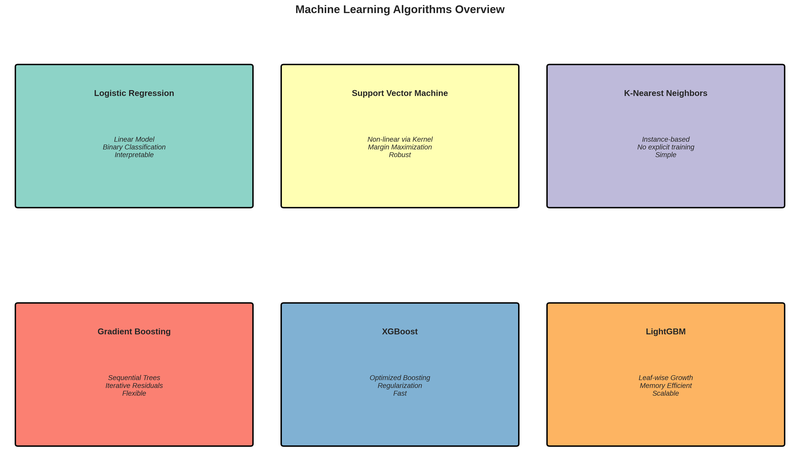
\includegraphics[width=0.9\textwidth]{perbandingan_algoritma.png}
\caption{Perbandingan Karakteristik Algoritma \eng{Machine Learning}}
\label{fig:perbandingan-algoritma}
\end{figure}

Gambar \ref{fig:perbandingan-algoritma} menunjukkan perbedaan karakteristik antara algoritma \eng{baseline} dan algoritma berbasis \eng{boosting}. Algoritma \eng{baseline} seperti \eng{Logistic Regression}, SVM, dan KNN umumnya lebih sederhana dan mudah diinterpretasikan, namun memiliki keterbatasan dalam menangani hubungan non-linear yang kompleks. Sebaliknya, algoritma \eng{boosting} seperti \eng{Gradient Boosting}, XGBoost, dan LightGBM mampu menangani data yang lebih kompleks melalui pendekatan \eng{ensemble}, sehingga cenderung menghasilkan performa prediksi yang lebih tinggi \cite{ref31}.

\subsection{Normalisasi Data}
Normalisasi data merupakan proses transformasi nilai pada fitur numerik ke dalam skala tertentu sehingga setiap variabel memiliki distribusi atau rentang nilai yang lebih seragam. Proses ini bertujuan untuk mengurangi perbedaan skala antar fitur, sehingga setiap variabel memiliki kontribusi yang seimbang dalam proses pembelajaran model \cite{ref32}. Perbedaan skala yang terlalu besar antar fitur dapat menyebabkan algoritma \eng{machine learning} menjadi bias terhadap fitur tertentu yang memiliki nilai dominan, sehingga berpotensi menurunkan performa model.

Normalisasi umumnya diterapkan pada algoritma yang sensitif terhadap skala data, seperti KNN, SVM, \eng{Neural Network}, serta metode berbasis \eng{clustering}. Salah satu metode yang digunakan dalam penelitian ini adalah \eng{Standard Scaler} atau standarisasi berbasis Z-score. Rumusnya dinyatakan sebagai:
\begin{equation}
 z = \frac{x-\mu}{\sigma},
 \label{eq:zscore}
\end{equation}
dengan $x$ menyatakan nilai data, $\mu$ sebagai rata-rata, $\sigma$ sebagai standar deviasi, dan $z$ merupakan hasil transformasi \cite{ref32}.

\subsection{Logistic Regression}
\eng{Logistic Regression} merupakan algoritma klasifikasi berbasis model linear yang digunakan untuk memprediksi probabilitas suatu data termasuk ke dalam kelas tertentu. Algoritma ini menggunakan fungsi sigmoid untuk mengubah keluaran linear menjadi nilai probabilitas antara 0 dan 1 \cite{ref11}. Fungsi sigmoid dinyatakan sebagai:
\begin{equation}
 \sigma(z)=\frac{1}{1+e^{-z}},
 \label{eq:sigmoid}
\end{equation}
dengan $z=\mathbf{w}^{T}\mathbf{x}+b$, di mana $\mathbf{w}$ merupakan bobot, $\mathbf{x}$ adalah fitur masukan, dan $b$ merupakan bias.

Keunggulan utama algoritma ini adalah interpretabilitas yang tinggi, karena setiap koefisien dapat menjelaskan pengaruh masing-masing fitur terhadap hasil prediksi. Namun, \eng{Logistic Regression} memiliki keterbatasan dalam menangani hubungan non-linear dan cenderung memiliki performa lebih rendah dibandingkan algoritma kompleks pada data dengan pola yang tidak sederhana \cite{ref10}.

\subsection{SVM}
\eng{Support Vector Machine} (SVM) merupakan algoritma klasifikasi yang bekerja dengan mencari \eng{hyperplane} terbaik untuk memisahkan dua kelas dengan margin maksimum. Jarak antara data terdekat dari masing-masing kelas atau \eng{support vectors} terhadap \eng{hyperplane} dibuat semaksimal mungkin \cite{ref11,ref33}. Fungsi keputusannya dapat dinyatakan sebagai:
\begin{equation}
 f(x)=\operatorname{sign}\left(\mathbf{w}\cdot\phi(x)+b\right),
 \label{eq:svm}
\end{equation}
dengan $\mathbf{w}$ adalah vektor bobot, $\phi(x)$ merupakan transformasi fitur melalui \eng{kernel}, dan $b$ adalah bias.

Keunggulan SVM terletak pada kemampuannya menangani data berdimensi tinggi dan menghasilkan margin optimal. Kelemahannya adalah waktu komputasi relatif tinggi pada dataset besar, serta kebutuhan pemilihan \eng{kernel} dan parameter yang tepat \cite{ref10}.

\subsection{KNN}
KNN merupakan algoritma berbasis \eng{instance-based learning} yang melakukan klasifikasi berdasarkan kedekatan jarak antar data. Algoritma ini menyimpan seluruh data latih dan menentukan kelas data baru berdasarkan mayoritas kelas dari tetangga terdekat \cite{ref14}. Jarak Euclidean dinyatakan sebagai:
\begin{equation}
 d(\mathbf{x},\mathbf{y})=\sqrt{\sum_{i=1}^{k}(x_i-y_i)^2}.
 \label{eq:euclidean}
\end{equation}
KNN sederhana dan mudah diimplementasikan, tetapi sensitif terhadap \eng{noise}, skala data, dan pemilihan nilai $k$. Tahap prediksi juga dapat memerlukan komputasi besar pada dataset berukuran besar \cite{ref14,ref34}.

\subsection{Gradient Boosting}
\eng{Gradient Boosting} bekerja dengan membangun model secara iteratif berdasarkan kesalahan atau residual model sebelumnya. Pada setiap iterasi, model baru dilatih untuk meminimalkan fungsi \eng{loss} dengan mengikuti arah gradien dari kesalahan yang dihasilkan \cite{ref35}. Proses tersebut dinyatakan sebagai:
\begin{equation}
 F_m(x)=F_{m-1}(x)+\gamma_m h_m(x),
 \label{eq:gradient-boosting}
\end{equation}
dengan $F_m(x)$ merupakan model pada iterasi ke-$m$, $h_m(x)$ adalah \eng{weak learner}, dan $\gamma_m$ adalah faktor pengali atau \eng{learning rate}. Algoritma ini mampu menangani hubungan non-linear, tetapi rentan \eng{overfitting} apabila parameternya tidak diatur dengan baik \cite{ref35}.

\subsection{XGBoost}
XGBoost merupakan pengembangan dari \eng{Gradient Boosting} yang dirancang untuk meningkatkan efisiensi dan performa melalui optimasi komputasi dan regularisasi \cite{ref36}. Fungsi objektifnya dapat dinyatakan sebagai:
\begin{equation}
 \mathrm{Obj}=\sum_i l(y_i,\hat{y}_i)+\sum_k\Omega(f_k),
 \label{eq:xgboost}
\end{equation}
dengan $l$ merupakan fungsi kerugian dan $\Omega$ adalah komponen regularisasi. XGBoost memiliki keunggulan dalam kecepatan pelatihan, generalisasi, dan ketahanan terhadap \eng{overfitting}, tetapi memerlukan \eng{hyperparameter tuning} yang lebih intensif dan interpretasinya lebih sulit \cite{ref36}.

\subsection{LightGBM}
LightGBM merupakan algoritma \eng{boosting} yang dikembangkan untuk meningkatkan efisiensi pelatihan, khususnya pada dataset besar. Berbeda dari pendekatan \eng{level-wise}, LightGBM menggunakan pertumbuhan pohon \eng{leaf-wise}, yaitu mengembangkan simpul yang memiliki kesalahan terbesar. LightGBM juga memanfaatkan \eng{Gradient-based One-Side Sampling} (GOSS) dan \eng{Exclusive Feature Bundling} (EFB) \cite{ref13}. Nilai \eng{gain} pada fitur ke-$j$ dengan titik \eng{split} $d$ dapat diringkas sebagai:
\begin{equation}
 V_{j\mid O}(d)=\frac{1}{n_O}\left(
 \frac{\left(\sum_{i\in O:x_{ij}\le d}g_i\right)^2}{n^{j}_{l\mid O}(d)}+
 \frac{\left(\sum_{i\in O:x_{ij}>d}g_i\right)^2}{n^{j}_{r\mid O}(d)}
 \right).
 \label{eq:lightgbm}
\end{equation}

\subsection{Optuna Framework}
\eng{Hyperparameter} merupakan parameter yang ditentukan sebelum proses pelatihan model dan sangat memengaruhi performa model \cite{ref18}. Optuna adalah kerangka optimasi \eng{hyperparameter} yang dikembangkan oleh Preferred Networks dan diperkenalkan pada 2019 \cite{ref37}. Optuna menggunakan pendekatan adaptif berbasis model probabilistik, secara bawaan menggunakan \eng{Tree-structured Parzen Estimator} (TPE), serta menyediakan mekanisme \eng{pruning} untuk menghentikan \eng{trial} yang tidak menjanjikan \cite{ref17}.

Salah satu karakteristik utama Optuna adalah prinsip \eng{define-by-run API}, sehingga ruang pencarian dapat dibangun secara dinamis. Secara umum, optimasi \eng{hyperparameter} dinyatakan sebagai:
\begin{equation}
 x^{*}=\arg\min_{x\in X} f(x),
 \label{eq:optuna}
\end{equation}
dengan $x$ adalah kombinasi parameter dan $f(x)$ merupakan fungsi objektif yang mengevaluasi performa model.

\subsection{Metrik Evaluasi}
Metrik evaluasi digunakan untuk mengukur performa model terhadap data. Dalam klasifikasi, evaluasi tidak hanya berfokus pada akurasi, tetapi juga mempertimbangkan kemampuan mendeteksi masing-masing kelas, terutama pada data tidak seimbang \cite{ref16}.

\subsubsection{Confusion Matrix}
\eng{Confusion matrix} membandingkan hasil prediksi dengan nilai aktual dan terdiri dari \eng{True Positive} (TP), \eng{True Negative} (TN), \eng{False Positive} (FP), dan \eng{False Negative} (FN) \cite{ref20}.

\begin{figure}[H]
\centering
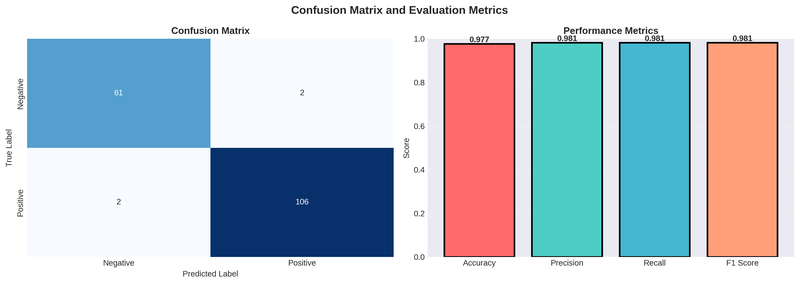
\includegraphics[width=0.88\textwidth]{confusion_matrix.png}
\caption{\eng{Confusion Matrix} dan \eng{Performance Metrics}}
\label{fig:confusion-matrix}
\end{figure}

Metrik yang dihitung dari \eng{confusion matrix} adalah:
\begin{align}
\mathrm{Accuracy} &= \frac{TP+TN}{TP+TN+FP+FN},\\
\mathrm{Precision} &= \frac{TP}{TP+FP},\\
\mathrm{Recall} &= \frac{TP}{TP+FN},\\
F1 &= 2\times\frac{\mathrm{Precision}\times\mathrm{Recall}}{\mathrm{Precision}+\mathrm{Recall}}.
\end{align}
Pada dataset tidak seimbang, \eng{precision}, \eng{recall}, dan \eng{F1-score} dapat memberikan gambaran yang lebih realistis dibandingkan akurasi saja \cite{ref16,ref38}.

\subsubsection{Kurva ROC dan AUC}
\eng{Receiver Operating Characteristic} (ROC) menunjukkan hubungan antara \eng{True Positive Rate} dan \eng{False Positive Rate} pada berbagai nilai ambang \cite{ref21}.

\begin{figure}[H]
\centering
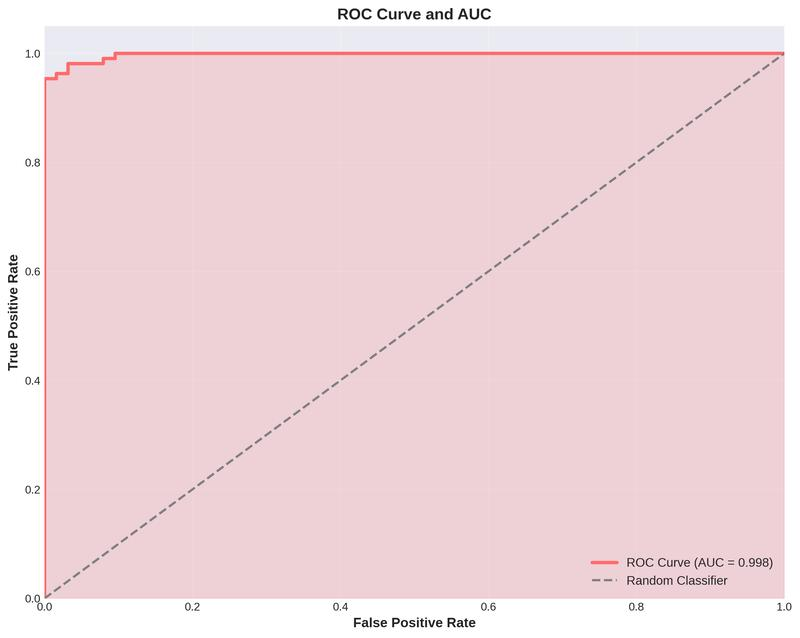
\includegraphics[width=0.78\textwidth]{roc_auc.png}
\caption{Kurva ROC dan AUC}
\label{fig:roc-auc}
\end{figure}

Nilai AUC yang mendekati 1 menunjukkan kemampuan klasifikasi yang semakin baik. Secara konseptual, AUC dapat dinyatakan sebagai:
\begin{equation}
 \mathrm{AUC}=\int_{0}^{1}\mathrm{TPR}\left(\mathrm{FPR}^{-1}(x)\right)\,dx.
 \label{eq:auc}
\end{equation}
Teknik \eng{cross-validation} digunakan untuk memastikan model tidak bergantung pada satu pembagian data dan menghasilkan evaluasi yang lebih stabil \cite{ref19}.

\subsection{Explainable AI}
Dalam penerapan \eng{machine learning} di bidang kesehatan, interpretabilitas model sangat penting. Model dengan akurasi tinggi tetapi sulit dipahami dapat sulit diterapkan dalam praktik klinis \cite{ref23}. \eng{Explainable AI} dikembangkan untuk meningkatkan transparansi model. Salah satu metode yang banyak digunakan adalah SHAP (SHAPley Additive exPlanations), yang menjelaskan kontribusi setiap fitur terhadap hasil prediksi \cite{ref24}. SHAP bersifat \eng{model-agnostic} dan dapat memberikan interpretasi lokal maupun global \cite{ref15}.

\begin{figure}[H]
\centering
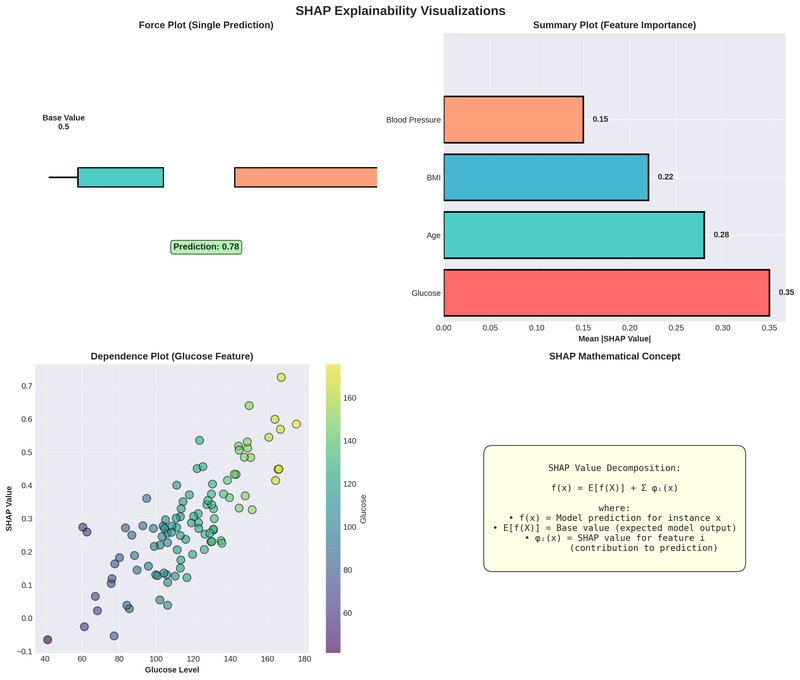
\includegraphics[width=0.9\textwidth]{shap_visualizations.png}
\caption{Visualisasi SHAP}
\label{fig:shap}
\end{figure}

Gambar \ref{fig:shap} menunjukkan beberapa visualisasi SHAP, seperti \eng{force plot}, \eng{summary plot}, dan \eng{dependence plot}. Secara matematis, prediksi dapat dinyatakan sebagai:
\begin{equation}
 f(x)=\phi_0+\sum_{i=1}^{n}\phi_i,
 \label{eq:shap}
\end{equation}
dengan $\phi_i$ menyatakan kontribusi fitur ke-$i$ dan $\phi_0$ merupakan nilai dasar prediksi. Meskipun demikian, SHAP memiliki keterbatasan, antara lain sensitivitas terhadap distribusi data dan asumsi independensi fitur, sehingga interpretasi perlu dilakukan secara hati-hati \cite{ref25}.

\chapter{Metode Penelitian}

Pada bab ini dijelaskan mengenai metode yang digunakan dalam penelitian, meliputi subjek dan objek penelitian, alat dan bahan yang digunakan, serta alur penelitian yang dilakukan secara sistematis.

\section{Subjek dan Objek Penelitian}
Dalam penelitian ini, subjek dan objek penelitian didefinisikan untuk memperjelas ruang lingkup serta fokus kajian yang dilakukan. Pada bidang sains data, subjek penelitian umumnya berupa data, algoritma, atau sistem yang digunakan dalam proses analisis dan pemodelan, bukan melibatkan partisipasi manusia secara langsung.

Subjek dalam penelitian ini adalah dataset diabetes yang digunakan sebagai sumber data utama dalam proses analisis dan pemodelan \eng{machine learning}. Dataset tersebut berisi berbagai atribut yang berkaitan dengan kondisi kesehatan individu, seperti kadar glukosa, tekanan darah, BMI, usia, serta variabel lain yang relevan dalam menentukan risiko T2DM. Selain data, subjek penelitian juga mencakup algoritma \eng{machine learning} yang digunakan, yaitu algoritma \eng{baseline} (\eng{Logistic Regression}, SVM, dan KNN) serta algoritma \eng{boosting} (\eng{Gradient Boosting}, XGBoost, dan LightGBM).

Sementara itu, objek penelitian dalam penelitian ini adalah performa model \eng{machine learning} dalam melakukan prediksi T2DM. Fokus utama penelitian adalah menganalisis dan membandingkan kinerja berbagai algoritma dalam mengklasifikasikan risiko diabetes, termasuk pengaruh \eng{hyperparameter tuning} terhadap peningkatan performa model, serta bagaimana interpretasi model dapat dilakukan menggunakan pendekatan XAI. Dengan demikian, penelitian ini berfokus pada bagaimana kombinasi algoritma, teknik optimasi, dan interpretasi model dapat menghasilkan sistem prediksi yang akurat dan dapat dipahami, khususnya dalam konteks data kesehatan.

\section{Alat dan Bahan Penelitian}

\subsection{Alat Penelitian}
Alat yang digunakan dalam penelitian ini terdiri dari perangkat keras dan perangkat lunak yang mendukung proses pengolahan data serta pemodelan \eng{machine learning}. Rinciannya adalah sebagai berikut:
\begin{enumerate}
\item \textbf{Perangkat keras}
  \begin{enumerate}[label=\alph*.]
  \item Laptop Asus Vivobook M1403QA.
  \item Prosesor AMD Ryzen 7 5800H with Radeon Graphics.
  \item Memori (RAM) 16 GB.
  \item Penyimpanan SSD 512 GB.
  \end{enumerate}
\item \textbf{Perangkat lunak}
  \begin{enumerate}[label=\alph*.]
  \item Visual Studio Code sebagai lingkungan pengembangan.
  \item Microsoft Word untuk penyusunan laporan penelitian.
  \item Microsoft Excel untuk pengolahan data awal.
  \item Mendeley sebagai manajemen referensi.
  \end{enumerate}
\end{enumerate}

\subsection{Bahan Penelitian}
Bahan penelitian yang digunakan adalah dataset EHR dari kompetisi \eng{Practice Fusion Diabetes Classification} yang diselenggarakan melalui Kaggle pada 2012 sebagai bagian dari \eng{data mining challenge} di bidang kesehatan yang berfokus pada prediksi T2DM. Dataset ini berasal dari Practice Fusion yang menyediakan data rekam medis pasien untuk keperluan analisis dan pengembangan model prediksi penyakit.

Dataset terdiri dari beberapa berkas utama, yaitu \texttt{diagnosis.csv} sebanyak 9.948 data, \texttt{medication.csv} sebanyak 9.836 data, \texttt{patient.csv} sebanyak 9.948 data, dan \texttt{transcript.csv} sebanyak 9.948 data. Berkas tersebut memuat informasi kondisi pasien, riwayat pengobatan, data demografis, spesialisasi dokter, serta catatan medis pasien. Variabel target penelitian adalah status diagnosis diabetes.

\section{Diagram Alir Penelitian}
Penelitian ini menggunakan pendekatan OSEMN (\eng{Obtain, Scrub, Explore, Model, iNterpret}) sebagai kerangka kerja dalam proses pengolahan data dan pembangunan model \eng{machine learning}. Pendekatan ini dipilih karena mampu menggambarkan alur kerja sains data secara sistematis, mulai dari pengumpulan data hingga interpretasi hasil model.

\begin{figure}[H]
\centering
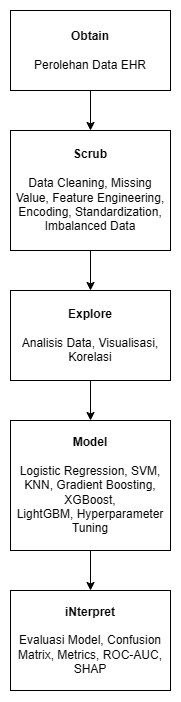
\includegraphics[height=0.68\textheight]{diagram_osemn.png}
\caption{Diagram Alir Penelitian}
\label{fig:diagram-osemn}
\end{figure}

\subsection{OBTAIN (Perolehan Data)}
Tahap \eng{Obtain} merupakan tahap awal dalam kerangka kerja OSEMN yang bertujuan memperoleh data yang relevan dengan tujuan penelitian, yaitu membangun model prediksi T2DM berbasis data EHR. Pada tahap ini dilakukan identifikasi sumber data, pemahaman struktur dataset, serta penentuan variabel yang akan digunakan dalam proses pemodelan \eng{machine learning}.

Dataset yang digunakan terdiri dari beberapa berkas utama yang merepresentasikan berbagai aspek rekam medis pasien. Untuk menghasilkan dataset yang komprehensif, seluruh data diintegrasikan menggunakan atribut kunci \texttt{PatientGuid}. Ringkasan struktur dataset disajikan pada Tabel \ref{tab:struktur-dataset}.

\begin{table}[H]
\centering
\caption{Struktur Dataset}
\label{tab:struktur-dataset}
\small
\begin{tabularx}{\textwidth}{|L{3cm}|Y|Y|}
\hline
\textbf{Dataset} & \textbf{Deskripsi} & \textbf{Atribut}\\ \hline
\texttt{patient.csv} & Data demografis pasien dan variabel target. Deskripsi lengkap disajikan pada Lampiran 1. & \texttt{PatientGuid}, \texttt{Age}, \texttt{Gender}, \texttt{State}, \texttt{DMIndicator}.\\ \hline
\texttt{diagnosis.csv} & Riwayat diagnosis berdasarkan ICD-9. Deskripsi lengkap disajikan pada Lampiran 2. & \texttt{PatientGuid}, \texttt{DiagnosisCount}, \texttt{VisitCount}, \texttt{DiagnosisFreq}, \texttt{AcuteCount}, \texttt{AcuteFreq}, dan kelompok \texttt{Icd9\_001-899}.\\ \hline
\texttt{medication.csv} & Data penggunaan obat pasien. Deskripsi lengkap disajikan pada Lampiran 3. & Fitur penggunaan obat pasien yang merepresentasikan konsumsi berbagai jenis obat, dengan jumlah atribut lebih dari 2.000 kolom.\\ \hline
\texttt{transcript.csv} & Data pemeriksaan klinis. Deskripsi lengkap disajikan pada Lampiran 4. & BMI (mean, max, min), tekanan darah sistolik dan diastolik, berat badan, suhu tubuh, serta fitur perubahan.\\ \hline
\end{tabularx}
\end{table}

Berdasarkan Tabel \ref{tab:struktur-dataset}, dataset mencakup data demografis, riwayat diagnosis, penggunaan obat, dan hasil pemeriksaan klinis. Dataset \texttt{patient.csv} berfungsi sebagai sumber utama karena memuat variabel target, sedangkan dataset lainnya berperan sebagai variabel prediktor yang memperkaya informasi pasien. Seluruh dataset diintegrasikan secara bertahap menggunakan \texttt{PatientGuid} sebagai kunci penggabungan.

\subsection{SCRUB (Pembersihan dan Penyiapan Data)}
Tahap \eng{Scrub} merupakan proses pembersihan dan penyiapan data agar siap digunakan dalam analisis dan pemodelan. Dataset EHR umumnya memiliki karakteristik kompleks, seperti adanya \eng{missing values}, data duplikat, serta distribusi kelas yang tidak seimbang. Kualitas data pada tahap ini akan memengaruhi performa model yang dihasilkan.

\subsubsection{Data Cleaning}
Pembersihan data dilakukan dengan memeriksa \eng{missing values}, data duplikat, dan konsistensi nilai pada setiap fitur. Pada data EHR, nilai hilang tidak selalu merupakan kesalahan karena dapat merepresentasikan pemeriksaan yang tidak dilakukan. Nilai hilang pada fitur numerik diimputasi menggunakan median karena lebih tahan terhadap \eng{outlier} dibandingkan rata-rata. Selain itu, ditambahkan \eng{missing indicator} agar model dapat menangkap informasi bahwa suatu nilai merupakan hasil imputasi. Data duplikat diidentifikasi dan dihapus, sedangkan \eng{outlier} diperiksa berdasarkan konteks klinis dan distribusi fitur.

\subsubsection{Feature Engineering dan Encoding}
Variabel kategorikal dikonversi menjadi numerik menggunakan \eng{one-hot encoding}, khususnya pada fitur nominal seperti jenis kelamin dan kategori diagnosis. Tipe data setiap fitur juga disesuaikan dengan kebutuhan model.

Fitur numerik kontinu distandarisasi menggunakan \eng{StandardScaler} untuk menyamakan skala antarvariabel. Proses ini diterapkan pada usia, BMI, tekanan darah, suhu tubuh, jumlah diagnosis, dan jumlah kunjungan. Fitur biner seperti kelompok ICD dan indikator penggunaan obat tidak distandarisasi. Bagi algoritma berbasis pohon, standarisasi bukan kebutuhan utama, tetapi tetap dimasukkan dalam \eng{pipeline} yang sesuai agar perbandingan antarmodel tetap konsisten.

\subsubsection{Pembagian Data}
Dataset dibagi menjadi data latih dan data uji dengan metode \eng{stratified split} pada proporsi 70:30. Data latih digunakan untuk pelatihan dan \eng{hyperparameter tuning}, sedangkan data uji digunakan secara eksklusif untuk evaluasi akhir. Pemisahan ini dilakukan untuk mencegah \eng{data leakage} dan menilai kemampuan generalisasi model terhadap data baru.

\subsubsection{Penanganan Class Imbalance}
Distribusi kelas pada dataset kesehatan sering tidak seimbang karena jumlah data non-diabetes dapat lebih besar dibandingkan data T2DM. Pendekatan yang digunakan meliputi penyesuaian \eng{class weight} pada model dan teknik \eng{oversampling} seperti SMOTE. Pemilihan metode dilakukan berdasarkan hasil evaluasi agar model tidak hanya akurat secara keseluruhan, tetapi juga mampu mendeteksi kelas diabetes dengan baik.

\subsection{EXPLORE (Eksplorasi Data)}
Tahap \eng{Explore} bertujuan memahami karakteristik data melalui \eng{Exploratory Data Analysis} (EDA) sebelum pemodelan. Analisis dilakukan menggunakan statistik deskriptif dan visualisasi untuk mengidentifikasi distribusi data, pola hubungan antarvariabel, serta indikasi awal faktor-faktor yang berpengaruh terhadap status T2DM.

\subsubsection{Analisis Distribusi Kelas}
Analisis distribusi kelas dilakukan dengan menghitung jumlah dan persentase kelas diabetes dan non-diabetes serta mengidentifikasi adanya \eng{class imbalance}. Hasil analisis digunakan untuk menentukan strategi penanganan ketidakseimbangan data dan metrik evaluasi yang sesuai.

\subsubsection{Statistik Deskriptif Variabel}
Statistik deskriptif digunakan untuk menggambarkan nilai rata-rata, minimum, maksimum, standar deviasi, dan distribusi fitur utama seperti BMI, tekanan darah, dan indikator klinis lainnya. Histogram dan \eng{boxplot} digunakan untuk memahami sebaran data serta mendeteksi potensi anomali atau \eng{outlier}.

\subsubsection{Analisis Hubungan Antarvariabel}
Analisis dilakukan untuk mengidentifikasi hubungan antara variabel prediktor dan status diabetes serta hubungan antarf fitur. Pendekatan yang digunakan bersifat deskriptif, misalnya membandingkan distribusi fitur pada kelompok diabetes dan non-diabetes dan menggunakan \eng{heatmap} korelasi. Analisis ini tidak digunakan untuk menarik kesimpulan kausal.

\subsection{MODEL (Pemodelan)}
Tahap \eng{Model} merupakan tahap inti yang bertujuan membangun model klasifikasi untuk memprediksi status T2DM berdasarkan data EHR. Dua kelompok algoritma digunakan, yaitu algoritma \eng{baseline} dan algoritma \eng{boosting}. Algoritma \eng{baseline} terdiri atas \eng{Logistic Regression}, SVM, dan KNN, sedangkan algoritma \eng{boosting} terdiri atas \eng{Gradient Boosting}, XGBoost, dan LightGBM.

Penggunaan dua kelompok tersebut bertujuan melihat peningkatan performa yang dihasilkan pendekatan \eng{ensemble} dibandingkan metode dasar. Seluruh pelatihan dan optimasi dilakukan hanya pada data latih, sedangkan data uji digunakan untuk evaluasi akhir.

\subsubsection{Desain Eksperimen}
Enam algoritma dilatih menggunakan dataset, variabel prediktor, dan pembagian data yang sama. Metrik evaluasi yang seragam digunakan agar perbandingan performa bersifat adil. Variabel prediktor berasal dari data demografis, kondisi klinis, riwayat diagnosis, penggunaan obat, dan indikator kesehatan lainnya, sedangkan target adalah status diabetes.

\subsubsection{Pipeline Pemodelan}
Gambar \ref{fig:pipeline-ml} menunjukkan alur proses pembangunan model \eng{machine learning} untuk prediksi Diabetes Mellitus Tipe 2.

\begin{figure}[H]
\centering
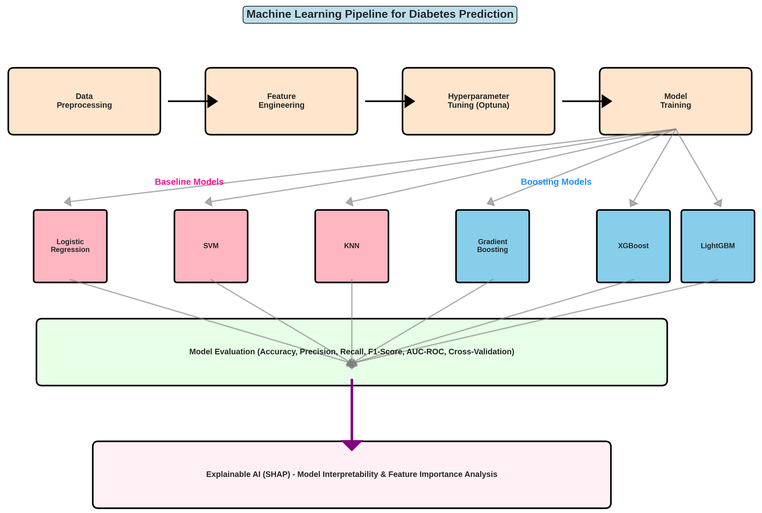
\includegraphics[width=0.98\textwidth]{pipeline_ml.png}
\caption{\eng{Machine Learning Pipeline} untuk Prediksi Diabetes}
\label{fig:pipeline-ml}
\end{figure}

Proses dimulai dari \eng{data preprocessing}, dilanjutkan dengan \eng{feature engineering}, pembentukan variabel prediktor $X$ dan target $Y$, serta pembagian data secara \eng{stratified}. Optuna digunakan untuk menemukan kombinasi \eng{hyperparameter} terbaik. Model kemudian dilatih dan dievaluasi menggunakan \eng{accuracy}, \eng{precision}, \eng{recall}, \eng{F1-score}, ROC-AUC, dan \eng{cross-validation}. Model terbaik selanjutnya dianalisis menggunakan SHAP.

\subsubsection{Baseline Model}
Model \eng{baseline} digunakan untuk memperoleh gambaran performa awal. \eng{Logistic Regression} dipilih karena sederhana dan memiliki interpretasi yang baik, SVM dipilih karena kemampuannya menangani data berdimensi tinggi, sedangkan KNN digunakan sebagai metode berbasis jarak yang sederhana.

\subsubsection{Model Boosting}
Model \eng{boosting} yang digunakan adalah \eng{Gradient Boosting}, XGBoost, dan LightGBM. \eng{Gradient Boosting} meminimalkan fungsi \eng{loss} secara iteratif, XGBoost menambahkan regularisasi dan optimasi komputasi, sedangkan LightGBM menggunakan pertumbuhan pohon \eng{leaf-wise} untuk mempercepat pelatihan pada dataset besar.

\subsubsection{Tuning Hyperparameter}
Optuna digunakan untuk mengoptimalkan parameter setiap algoritma. Parameter yang ditelusuri antara lain:
\begin{itemize}
\item \eng{Logistic Regression}: parameter regularisasi.
\item SVM: jenis \eng{kernel}, parameter $C$, dan parameter kernel.
\item KNN: jumlah tetangga $k$, bobot, dan metrik jarak.
\item \eng{Gradient Boosting}: \eng{learning rate}, jumlah estimator, dan kedalaman pohon.
\item XGBoost dan LightGBM: \eng{learning rate}, \eng{max depth}, jumlah pohon, subsampling, dan parameter regularisasi.
\end{itemize}

\subsubsection{Model Final dan Evaluasi}
Model final diperoleh dari kombinasi parameter terbaik pada masing-masing algoritma. Evaluasi dilakukan pada data uji menggunakan \eng{accuracy}, \eng{precision}, \eng{recall}, \eng{F1-score}, dan ROC-AUC. \eng{Cross-validation} digunakan pada tahap pelatihan untuk menilai kestabilan model dan mengidentifikasi potensi \eng{overfitting}. SHAP hanya diterapkan pada model dengan performa terbaik.

\subsection{INTERPRET (Evaluasi dan Interpretasi Model)}
Tahap \eng{iNterpret} merupakan tahap akhir yang bertujuan mengevaluasi performa model dan memahami hasil prediksi. Evaluasi dilakukan untuk mengukur kemampuan model mengklasifikasikan status T2DM, khususnya pada data yang berpotensi tidak seimbang. Interpretasi model digunakan agar hasil prediksi dapat dipahami dalam konteks kesehatan.

\subsubsection{Evaluasi Model}
Evaluasi model dilakukan pada data uji yang belum pernah dilihat selama pelatihan.

\paragraph{Confusion Matrix.}
Komponen yang dianalisis adalah:
\begin{itemize}
\item \eng{True Positive} (TP): data diabetes yang diprediksi benar sebagai diabetes.
\item \eng{True Negative} (TN): data non-diabetes yang diprediksi benar sebagai non-diabetes.
\item \eng{False Positive} (FP): data non-diabetes yang diprediksi sebagai diabetes.
\item \eng{False Negative} (FN): data diabetes yang diprediksi sebagai non-diabetes.
\end{itemize}

\paragraph{Metrik Evaluasi.}
\eng{Accuracy} digunakan untuk mengukur ketepatan keseluruhan, \eng{precision} untuk mengukur ketepatan prediksi kelas diabetes, \eng{recall} untuk mengukur kemampuan mendeteksi kasus diabetes, dan \eng{F1-score} untuk menyeimbangkan \eng{precision} dan \eng{recall}. Dalam konteks penelitian ini, \eng{recall} menjadi metrik penting karena berkaitan dengan minimisasi \eng{false negative}.

\paragraph{ROC-AUC.}
ROC-AUC digunakan untuk menilai kemampuan model membedakan kelas diabetes dan non-diabetes pada berbagai nilai ambang. \eng{Cross-validation} digunakan untuk memastikan hasil evaluasi tidak bergantung pada satu pembagian data.

\subsubsection{Interpretasi Model}
Metode SHAP diterapkan pada model dengan performa terbaik. Visualisasi yang digunakan meliputi:
\begin{itemize}
\item \eng{Summary plot} untuk menunjukkan fitur paling berpengaruh secara global.
\item \eng{Dependence plot} untuk menunjukkan hubungan nilai fitur dan pengaruhnya terhadap prediksi.
\item \eng{Force plot} untuk menjelaskan kontribusi fitur pada prediksi individu.
\end{itemize}

Keluaran tahap ini berupa perbandingan performa seluruh algoritma, penentuan model terbaik berdasarkan metrik evaluasi, serta visualisasi dan interpretasi kontribusi fitur menggunakan SHAP. Hasil tersebut digunakan untuk menarik kesimpulan mengenai model terbaik dan memahami faktor-faktor yang memengaruhi prediksi T2DM berdasarkan data EHR.


\clearpage
\phantomsection
\addcontentsline{toc}{chapter}{DAFTAR PUSTAKA}
\printbibliography[title={DAFTAR PUSTAKA}]

\clearpage
\chapter*{LAMPIRAN}
\addcontentsline{toc}{chapter}{LAMPIRAN}

\section*{Lampiran 1. Deskripsi Dataset \texttt{patient.csv}}
\label{app:patient}
\addcontentsline{toc}{section}{Lampiran 1. Deskripsi Dataset patient.csv}
\setlength{\tabcolsep}{3pt}
\begin{longtable}{|L{2.5cm}|C{1.8cm}|L{5.3cm}|L{3.5cm}|}
\hline
\textbf{Variabel} & \textbf{Tipe Data} & \textbf{Deskripsi} & \textbf{Keterangan}\\ \hline
\endfirsthead
\hline
\textbf{Variabel} & \textbf{Tipe Data} & \textbf{Deskripsi} & \textbf{Keterangan}\\ \hline
\endhead
\texttt{PatientGuid} & String & Identitas unik untuk setiap pasien yang digunakan sebagai kunci utama dalam proses penggabungan data. & ID alfanumerik.\\ \hline
\texttt{Age} & Integer & Usia pasien pada saat pencatatan data. & 0--120 tahun.\\ \hline
\texttt{Gender} & Kategorikal & Jenis kelamin pasien. & Male, Female, Unknown.\\ \hline
\texttt{State} & Kategorikal & Lokasi geografis pasien berdasarkan wilayah negara bagian. & Kode state (CA, TX, NY, dan lain-lain).\\ \hline
\texttt{DMIndicator} & Biner (Target) & Status diagnosis Diabetes Mellitus Tipe 2. & 1 = Diabetes, 0 = Non-diabetes.\\ \hline
\end{longtable}

\section*{Lampiran 2. Deskripsi Dataset \texttt{diagnosis.csv}}
\label{app:diagnosis}
\addcontentsline{toc}{section}{Lampiran 2. Deskripsi Dataset diagnosis.csv}
\small
\begin{longtable}{|L{2.7cm}|C{1.8cm}|L{5.1cm}|L{3.5cm}|}
\hline
\textbf{Variabel} & \textbf{Tipe Data} & \textbf{Deskripsi} & \textbf{Keterangan}\\ \hline
\endfirsthead
\hline
\textbf{Variabel} & \textbf{Tipe Data} & \textbf{Deskripsi} & \textbf{Keterangan}\\ \hline
\endhead
\texttt{PatientGuid} & String & Identitas unik pasien. & Digunakan sebagai kunci penggabungan data.\\ \hline
\texttt{Icd9\_001-139} & Biner (0/1) & Penyakit infeksi dan parasit (rentang ICD-9: 001--139). & Menunjukkan keberadaan diagnosis.\\ \hline
\texttt{Icd9\_140-239} & Biner (0/1) & Neoplasma (rentang ICD-9: 140--239). & Riwayat kanker atau tumor.\\ \hline
\texttt{Icd9\_240-279} & Biner (0/1) & Penyakit endokrin, nutrisi, dan metabolik. & Sangat relevan terhadap diabetes.\\ \hline
\texttt{Icd9\_280-289} & Biner (0/1) & Penyakit darah dan organ pembentuk darah. & Misalnya anemia.\\ \hline
\texttt{Icd9\_290-319} & Biner (0/1) & Gangguan mental, perilaku, dan perkembangan saraf. & Riwayat gangguan psikiatri.\\ \hline
\texttt{Icd9\_320-359} & Biner (0/1) & Penyakit sistem saraf. & Kondisi neurologis.\\ \hline
\texttt{Icd9\_360-389} & Biner (0/1) & Penyakit mata dan telinga. & Gangguan sistem sensorik.\\ \hline
\texttt{Icd9\_390-459} & Biner (0/1) & Penyakit sistem peredaran darah. & Berkaitan dengan hipertensi dan penyakit jantung.\\ \hline
\texttt{Icd9\_460-519} & Biner (0/1) & Penyakit sistem pernapasan. & Gangguan paru-paru.\\ \hline
\texttt{Icd9\_520-579} & Biner (0/1) & Penyakit sistem pencernaan. & Gangguan gastrointestinal.\\ \hline
\texttt{Icd9\_580-629} & Biner (0/1) & Penyakit sistem genitourinari. & Termasuk komplikasi ginjal.\\ \hline
\texttt{Icd9\_630-679} & Biner (0/1) & Komplikasi kehamilan, persalinan, dan masa nifas. & Kondisi obstetri.\\ \hline
\texttt{Icd9\_680-709} & Biner (0/1) & Penyakit kulit dan jaringan subkutan. & Gangguan kulit.\\ \hline
\texttt{Icd9\_710-739} & Biner (0/1) & Penyakit sistem muskuloskeletal. & Gangguan tulang dan sendi.\\ \hline
\texttt{Icd9\_740-759} & Biner (0/1) & Kelainan bawaan. & Cacat sejak lahir.\\ \hline
\texttt{Icd9\_760-779} & Biner (0/1) & Kondisi yang berasal dari periode perinatal. & Kondisi terkait kelahiran.\\ \hline
\texttt{Icd9\_780-799} & Biner (0/1) & Gejala, tanda, dan temuan abnormal. & Gejala non-spesifik.\\ \hline
\texttt{Icd9\_800-899} & Biner (0/1) & Cedera dan keracunan akibat faktor eksternal. & Riwayat trauma.\\ \hline
\texttt{Icd9\_E-V} & Biner (0/1) & Penyebab eksternal cedera dan klasifikasi tambahan. & Kode E dan V.\\ \hline
\texttt{Icd9\_Unknown} & Biner (0/1) & Kode diagnosis tidak diketahui atau tidak terklasifikasi. & Indikator kualitas data.\\ \hline
\texttt{DiagnosisCount} & Integer & Jumlah total diagnosis yang dimiliki pasien. & Menggambarkan beban penyakit.\\ \hline
\texttt{VisitCount} & Integer & Jumlah total kunjungan medis pasien. & Tingkat interaksi dengan layanan kesehatan.\\ \hline
\texttt{DiagnosisFreq} & Float & Rata-rata jumlah diagnosis per kunjungan. & Indikator kompleksitas klinis.\\ \hline
\texttt{AcuteCount} & Integer & Jumlah diagnosis akut (kondisi sementara). & Frekuensi penyakit akut.\\ \hline
\texttt{AcuteFreq} & Float & Rata-rata diagnosis akut per kunjungan. & Tingkat kejadian kondisi akut.\\ \hline
\end{longtable}
\normalsize

\section*{Lampiran 3. Deskripsi Dataset \texttt{medication.csv}}
\label{app:medication}
\addcontentsline{toc}{section}{Lampiran 3. Deskripsi Dataset medication.csv}
\small
\begin{longtable}{|L{2.8cm}|C{1.8cm}|L{3.3cm}|L{5.2cm}|}
\hline
\textbf{Variabel} & \textbf{Tipe Data} & \textbf{Deskripsi} & \textbf{Keterangan}\\ \hline
\endfirsthead
\hline
\textbf{Variabel} & \textbf{Tipe Data} & \textbf{Deskripsi} & \textbf{Keterangan}\\ \hline
\endhead
\texttt{PatientGuid} & String & Identitas unik pasien. & Digunakan sebagai kunci penggabungan data.\\ \hline
\texttt{Medication\_1} hingga \texttt{Medication\_n} & Biner (0/1) & Indikator apakah suatu obat pernah diresepkan kepada pasien. & Contoh: abacavir, abilify, acarbose, aceon, aciphex, acyclovir, adalimumab, adderall, advair, advil, albuterol, aldactone, aleve, allegra, allopurinol, amaryl, ambien, amiodarone, amitriptyline, amlodipine, amoxicillin, ampicillin, anastrozole, androgel, aspirin, atenolol, atorvastatin, azithromycin, furosemide, hydrochlorothiazide, ibuprofen, insulin, lantus, lisinopril, losartan, metformin, metoprolol, naproxen, omeprazole, pravastatin, simvastatin, spironolactone, dan lain-lain.\\ \hline
\texttt{DMIndicator} & Biner & Status diagnosis Diabetes Mellitus Tipe 2. & 1 = Diabetes, 0 = Non-diabetes.\\ \hline
\end{longtable}
\normalsize

\section*{Lampiran 4. Deskripsi Dataset \texttt{transcript.csv}}
\label{app:transcript}
\addcontentsline{toc}{section}{Lampiran 4. Deskripsi Dataset transcript.csv}
\scriptsize
\begin{longtable}{|L{2.8cm}|L{4.2cm}|L{3.5cm}|L{2.6cm}|}
\hline
\textbf{Kategori} & \textbf{Variabel} & \textbf{Deskripsi} & \textbf{Relevansi terhadap Diabetes}\\ \hline
\endfirsthead
\hline
\textbf{Kategori} & \textbf{Variabel} & \textbf{Deskripsi} & \textbf{Relevansi terhadap Diabetes}\\ \hline
\endhead
Anthropometric & \path{Height_Max, Height_Min, Height_Mean, Height_Std} & Tinggi badan pasien dalam berbagai nilai agregasi. & Digunakan sebagai dasar perhitungan BMI.\\ \hline
Anthropometric & \path{Weight_Max, Weight_Min, Weight_Mean, Weight_Std} & Berat badan pasien dalam berbagai nilai agregasi. & Faktor penting dalam risiko T2DM.\\ \hline
Anthropometric & \path{BMI_Max, BMI_Min, BMI_Mean, BMI_Std} & Indeks Massa Tubuh yang dihitung dari berat dan tinggi badan. & Prediktor utama risiko diabetes.\\ \hline
Anthropometric & \path{Weight_Change} & Perubahan berat badan antarkunjungan. & Indikator tren kondisi pasien.\\ \hline
Blood Pressure & \path{SystolicBP_Max, SystolicBP_Min, SystolicBP_Mean, SystolicBP_Std} & Tekanan darah sistolik dalam berbagai agregasi. & Berkaitan dengan risiko hipertensi.\\ \hline
Blood Pressure & \path{DiastolicBP_Max, DiastolicBP_Min, DiastolicBP_Mean, DiastolicBP_Std} & Tekanan darah diastolik dalam berbagai agregasi. & Indikator tambahan kondisi kardiovaskular.\\ \hline
Blood Pressure & \path{SystolicBP_Change, DiastolicBP_Change} & Perubahan tekanan darah antarwaktu. & Indikator perkembangan kondisi kesehatan.\\ \hline
Respiratory & \path{RespiratoryRate_Max, RespiratoryRate_Min, RespiratoryRate_Mean, RespiratoryRate_Std} & Laju pernapasan pasien. & Indikator kondisi kesehatan umum.\\ \hline
Respiratory & \path{RespiratoryRate_Change} & Perubahan laju pernapasan. & Indikator penurunan kondisi kesehatan.\\ \hline
Thermoregulation & \path{Temperature_Max, Temperature_Min, Temperature_Mean, Temperature_Std} & Suhu tubuh pasien. & Indikator infeksi atau inflamasi.\\ \hline
Thermoregulation & \path{Temperature_Change} & Perubahan suhu tubuh antarwaktu. & Indikator perubahan kondisi kesehatan.\\ \hline
Derived Metrics & \path{BMI_Change} & Perubahan BMI dari waktu ke waktu. & Penting untuk analisis tren risiko diabetes.\\ \hline
Derived Metrics & \path{Height_Change} & Perubahan tinggi badan. & Digunakan untuk pengecekan kualitas data.\\ \hline
\end{longtable}
\normalsize

\setlength{\tabcolsep}{6pt}


\end{document}
